\documentclass[12pt,prb,aps,epsf]{article}
\usepackage[utf8]{inputenc}
\usepackage{amsmath}
\usepackage{amsfonts}
\usepackage{amssymb}
\usepackage{graphicx} 
\usepackage{latexsym} 
\usepackage[toc,page]{appendix}
\usepackage{listings}
\usepackage{xcolor}
\usepackage{soul}
\usepackage[T1]{fontenc}
\usepackage{amsthm}
\usepackage{mathtools}
\usepackage{setspace}
\usepackage{array,multirow,makecell}
\usepackage{geometry}
\usepackage{textcomp}
\usepackage{float}
%\usepackage{siunitx}
\usepackage{cancel}
%\usepackage{tikz}
%\usetikzlibrary{calc, shapes, backgrounds, arrows, decorations.pathmorphing, positioning, fit, petri, tikzmark}
\usepackage{here}
\usepackage{titlesec}
%\usepackage{bm}
\usepackage{bbold}

\geometry{hmargin=2cm,vmargin=2cm}

\begin{document}
	
	\title{LP 45 Paramagnétisme, ferromagnétisme : approximation du champ moyen}
	\author{Naïmo Davier}
	
	\maketitle
	
	\tableofcontents
	
	\pagebreak
	
	
\section{Introduction}
\textit{Magnétisme I de E du Trémolet chapitre 1}\\
\textbf{Pré requis} : Électromagnétisme de 2e année, ensemble canonique, quantification de l'énergie et moment cinétique en mécanique quantique, thermodynamique.\\

Les propriétés magnétiques de certains matériaux ont été remarquées depuis quelques milliers d'années déjà, puisque par exemple au palais de Knossos en Crête, vieux d'environ 4000 ans, on a observé que le centre de la salle du trône du Minos était pavée en son centre de magnétite, qui ne devait donc sans doute pas se trouver là par hasard. Il aura cependant fallu attendre jusqu'au 19e s pour qu'on commence à étudier de près le magnétisme et la fin du 19e pour voir émerger des modèles satisfaisants pour décrire les comportements des matériaux ayant des propriétés magnétiques.\\
On va au cours de cette leçon exposer l'interprétation moderne que l'on fait de ces comportements, en utilisant tout l'attirail physique développé jusqu'ici.

\section{Notion de magnétisme}
\subsection{Aimantation}
\textit{Magnétisme I de E du Trémolet chapitre 2}\\

On va commencer par définir ici les grandeurs que nous allons utiliser tout au cours de cette leçon. L'aimantation est une propriété intrinsèque des matériaux, qui se manifeste notamment par l'induction d'un champ magnétique. On peut la caractériser soit à partir de densités volumiques de courants liés à la matière $\vec{j}_m$ au quel cas l'aimantation $\vec{M}$ se définit comme 
\begin{eqnarray}
\vec{j}_m = \vec{rot}\times \vec{M},
\end{eqnarray}  
soit comme étant une densité volumique de moment dipolaire $\vec{m}$, on la note alors $\vec{M}$, c'est le champ vectoriel défini par
\begin{eqnarray}
\vec{M} = \frac{d\vec{m}}{dV}
\end{eqnarray}
Le moment magnétique peut être quand à lui être défini de manière analogue au moment cinétique en mécanique, à partir du courant jouant le rôle de la vitesse en mécanique
\begin{eqnarray}
\vec{m} &=& \frac{1}{2}\int_{V}\vec{r}\times \vec{j}(\vec{r})\,d^3r\\
 &=& \frac{1}{2} \int_{\mathcal{C}} \vec{r}\times I\vec{dl}\hspace{1cm}\mathrm{dans\; le\; cas\; d'une\; boucle\;de\;courant}
\end{eqnarray}
On pourra noter enfin que l'énergie d'interaction d'un dipôle magnétique de moment $\vec{m}$ avec un champ $\vec{B}$ s'écrit 
\begin{eqnarray}
E = - \vec{m}.\vec{B}\hspace{1cm}\mathrm{associ\acute{e}\;a\;la\;force}\;\; \vec{F} = (\vec{m}.\vec{\nabla})\vec{B}
\end{eqnarray}

On va maintenant voir comment illustrer de manière plus concrète et visuelle la notion de moment magnétique avec le cas simple d'un électron orbitant autour d'un proton.

\subsection{Moment magnétique atomique}
\textit{Magnétisme I de E du Trémolet p249}\\

Si on considère le modèle de Bohr pour un atome quelconque, et que l'on regarde un électron orbitant à la vitesse $\vec{v}$ et à une distance $r$ autour du noyau on a alors 
\begin{eqnarray}
\vec{j}(\vec{r}') = -e\vec{v}\;\delta^{(3)}(\vec{r}-\vec{r}') 
\end{eqnarray}
ce qui mène à 
\begin{eqnarray}
\vec{m} = \frac{1}{2}\int_{V}\vec{r}'\times \vec{j}(\vec{r}')d^3r' = \frac{-e}{2}\vec{r}\times\vec{v} = -\frac{e}{2m_e}\vec{L}
\end{eqnarray}
où $\vec{L}$ est le moment cinétique de l'électron. On en déduit que les particules chargées ont un moment magnétique proportionnel à leur moment cinétique, le coefficient de proportionnalité étant le rapport gyromagnétique noté $\gamma$ et égal à $-\frac{e}{2m_e}$ dans le cas traité.\\  

Du point de vue quantique on conserve cette relation de proportionnalité mais cette fois comme vous le savez le moment cinétique est un opérateur, et au moment cinétique dû à l'orbite de la particule s'ajoute un moment cinétique intrinsèque : le spin.\\ %Pour rappel on peut alors définir une base des états pour le moment moment cinétique $|n,l,m,\sigma\rangle$ qui est associée aux valeurs propres 
%\begin{eqnarray}
%\hat{L}^2 |n,l,m,\sigma\rangle = \hbar l(l+1)|n,l,m,\sigma\rangle\\
%\hat{L}_z |n,l,m,\sigma\rangle = \hbar m |n,l,m,\sigma\rangle
%\end{eqnarray}

On a donc pu voir ici que l'aimantation des matériaux était due aux moments magnétiques portés par leurs atomes, ces derniers provenant du mouvement des électrons et de leur spin essentiellement.\\

On va, maintenant ces outils définis et illustrés, les utiliser pour rentrer dans le détail des notions qui nous intéressent.

\section{Paramagnétisme}
\subsection{Présentation}
Si on s'intéresse au cas général des matériaux il existe différents comportements magnétiques possibles à l'échelle atomique. Le premier, sans doute le plus courant est celui des matériaux composés d'atomes n'ayant pas de moment magnétique, dans ce cas si l'on soumet le matériau à un champ magnétique alors ce dernier va produire une aimantation, due aux courants initiés dans le solide selon la loi de Lenz, qui induit un champ s'opposant aux champs extérieurs. Dans ce cas l'aimantation est alors très faible et de sens opposée au champ, ces matériaux sont alors dits diamagnétiques\\

Si par contre les atomes composant le matériau possèdent des propriétés magnétiques alors il y a, en plus de la réponse précédente, une interaction entre les moments dipolaires des atomes et le champ d'énergie 
\begin{eqnarray}
\varepsilon_i = -\vec{m}_i.\vec{B}
\end{eqnarray}
On voit alors que cette fois cette interaction va amener l'aimantation à s'orienter dans la même direction que le champ, et cette dernière étant beaucoup plus intense que l'interaction vue plus haut pour les diamagnétiques elle va ici caractériser complètement ces matériaux, qui sont alors dits paramagnétiques.

\subsection{Description dans l'ensemble canonique}
Fait très proprement mais aussi un peu lourdement dans le \textit{complément III.A p309 du Diu de stat}\\
Moins propre mais plus parlant dans le \textit{Faroux Renault de thermo p261}\\


On considère un solide cristallin, constitué d'atomes ayant des moments magnétiques $\vec{m} = g\mu_B\vec{J}$ (avec g le facteur de Landé et $\mu_B=\gamma\hbar = \frac{\hbar e}{2m}$ le magnéton de Bohr) et à l'équilibre thermique avec l'extérieur, qui fait office de thermostat. On suppose ici que ces moments magnétiques n'interagissent pas entre eux ou alors très faiblement, on les considèrera donc comme indépendants. On va considérer le cas simple où les moments magnétiques n'ont que deux niveaux, cela revient à considérer le cas $j=\frac{1}{2}$ ou le cas d'un spin $\frac{1}{2}$. On a alors deux valeurs propres pour $m_z$ (avec l'axe $Oz$ défini par le champ magnétique extérieur) qui sont $\pm g\mu_B/2$, associées aux énergies propres $\varepsilon_{\mp}=\mp g\mu_B B/2 = \mp \varepsilon$ puisque le hamiltonien d'interaction entre le champ et les moments magnétiques est défini comme
\begin{eqnarray}
\hat{\mathcal{H}} = -\hat{\vec{m}}.\vec{B} = -g\mu_B\hat{J}_zB
\end{eqnarray}

On considère que notre système est à l'équilibre thermique à la température $T$ avec le thermostat, on a alors, en notant $N_+$ (resp $N_-$) le nombre d'atomes dans l'état d'énergie $\varepsilon_+$ (resp $\varepsilon_-$) et dans un volume V, que les probabilités d'occupation de ces états sont 
\begin{eqnarray}
P_+ = \frac{N_+}{N} = Ae^{-\beta\varepsilon_+}\hspace{1cm}\mathrm{et}\hspace{1cm}P_+ = \frac{N_-}{N} = Ae^{-\beta\varepsilon_-}
\end{eqnarray} 
où $\beta = 1/k_BT$, $N=N_++N_-$ et où $A$ est tel que $P_++P_- = 1$. On a alors 
\begin{eqnarray}
M_z = \frac{N_+}{V}m_z - \frac{N_-}{V}m_z = \frac{N}{V}m_z \frac{e^{\beta\varepsilon} - e^{-\beta\varepsilon}}{e^{\beta\varepsilon}+e^{-\beta\varepsilon}} = \frac{Ng\mu_B}{2V}\mathrm{tanh}\left(\frac{\beta g\mu_B B}{2}\right)
\end{eqnarray}
Si on considère qu'à l'équilibre tous les moments ont relaxés jusqu'à être alignés sur l'axe défini par le champ on a alors 
\begin{eqnarray}
M = M_z  = M_s \mathrm{tanh}\left(\frac{g\mu_B B}{2k_BT}\right)
\end{eqnarray}
cette équation est l'équation d'état d'un système de spins, reliant à l'équilibre l'aimantation aux variables externes $B$ et $T$. Dans le cas général $j\neq\frac{1}{2}$ on a une expression plus compliquée mais comparable représentée sur la figure ci dessous.

\begin{figure}[h]
	\centerline{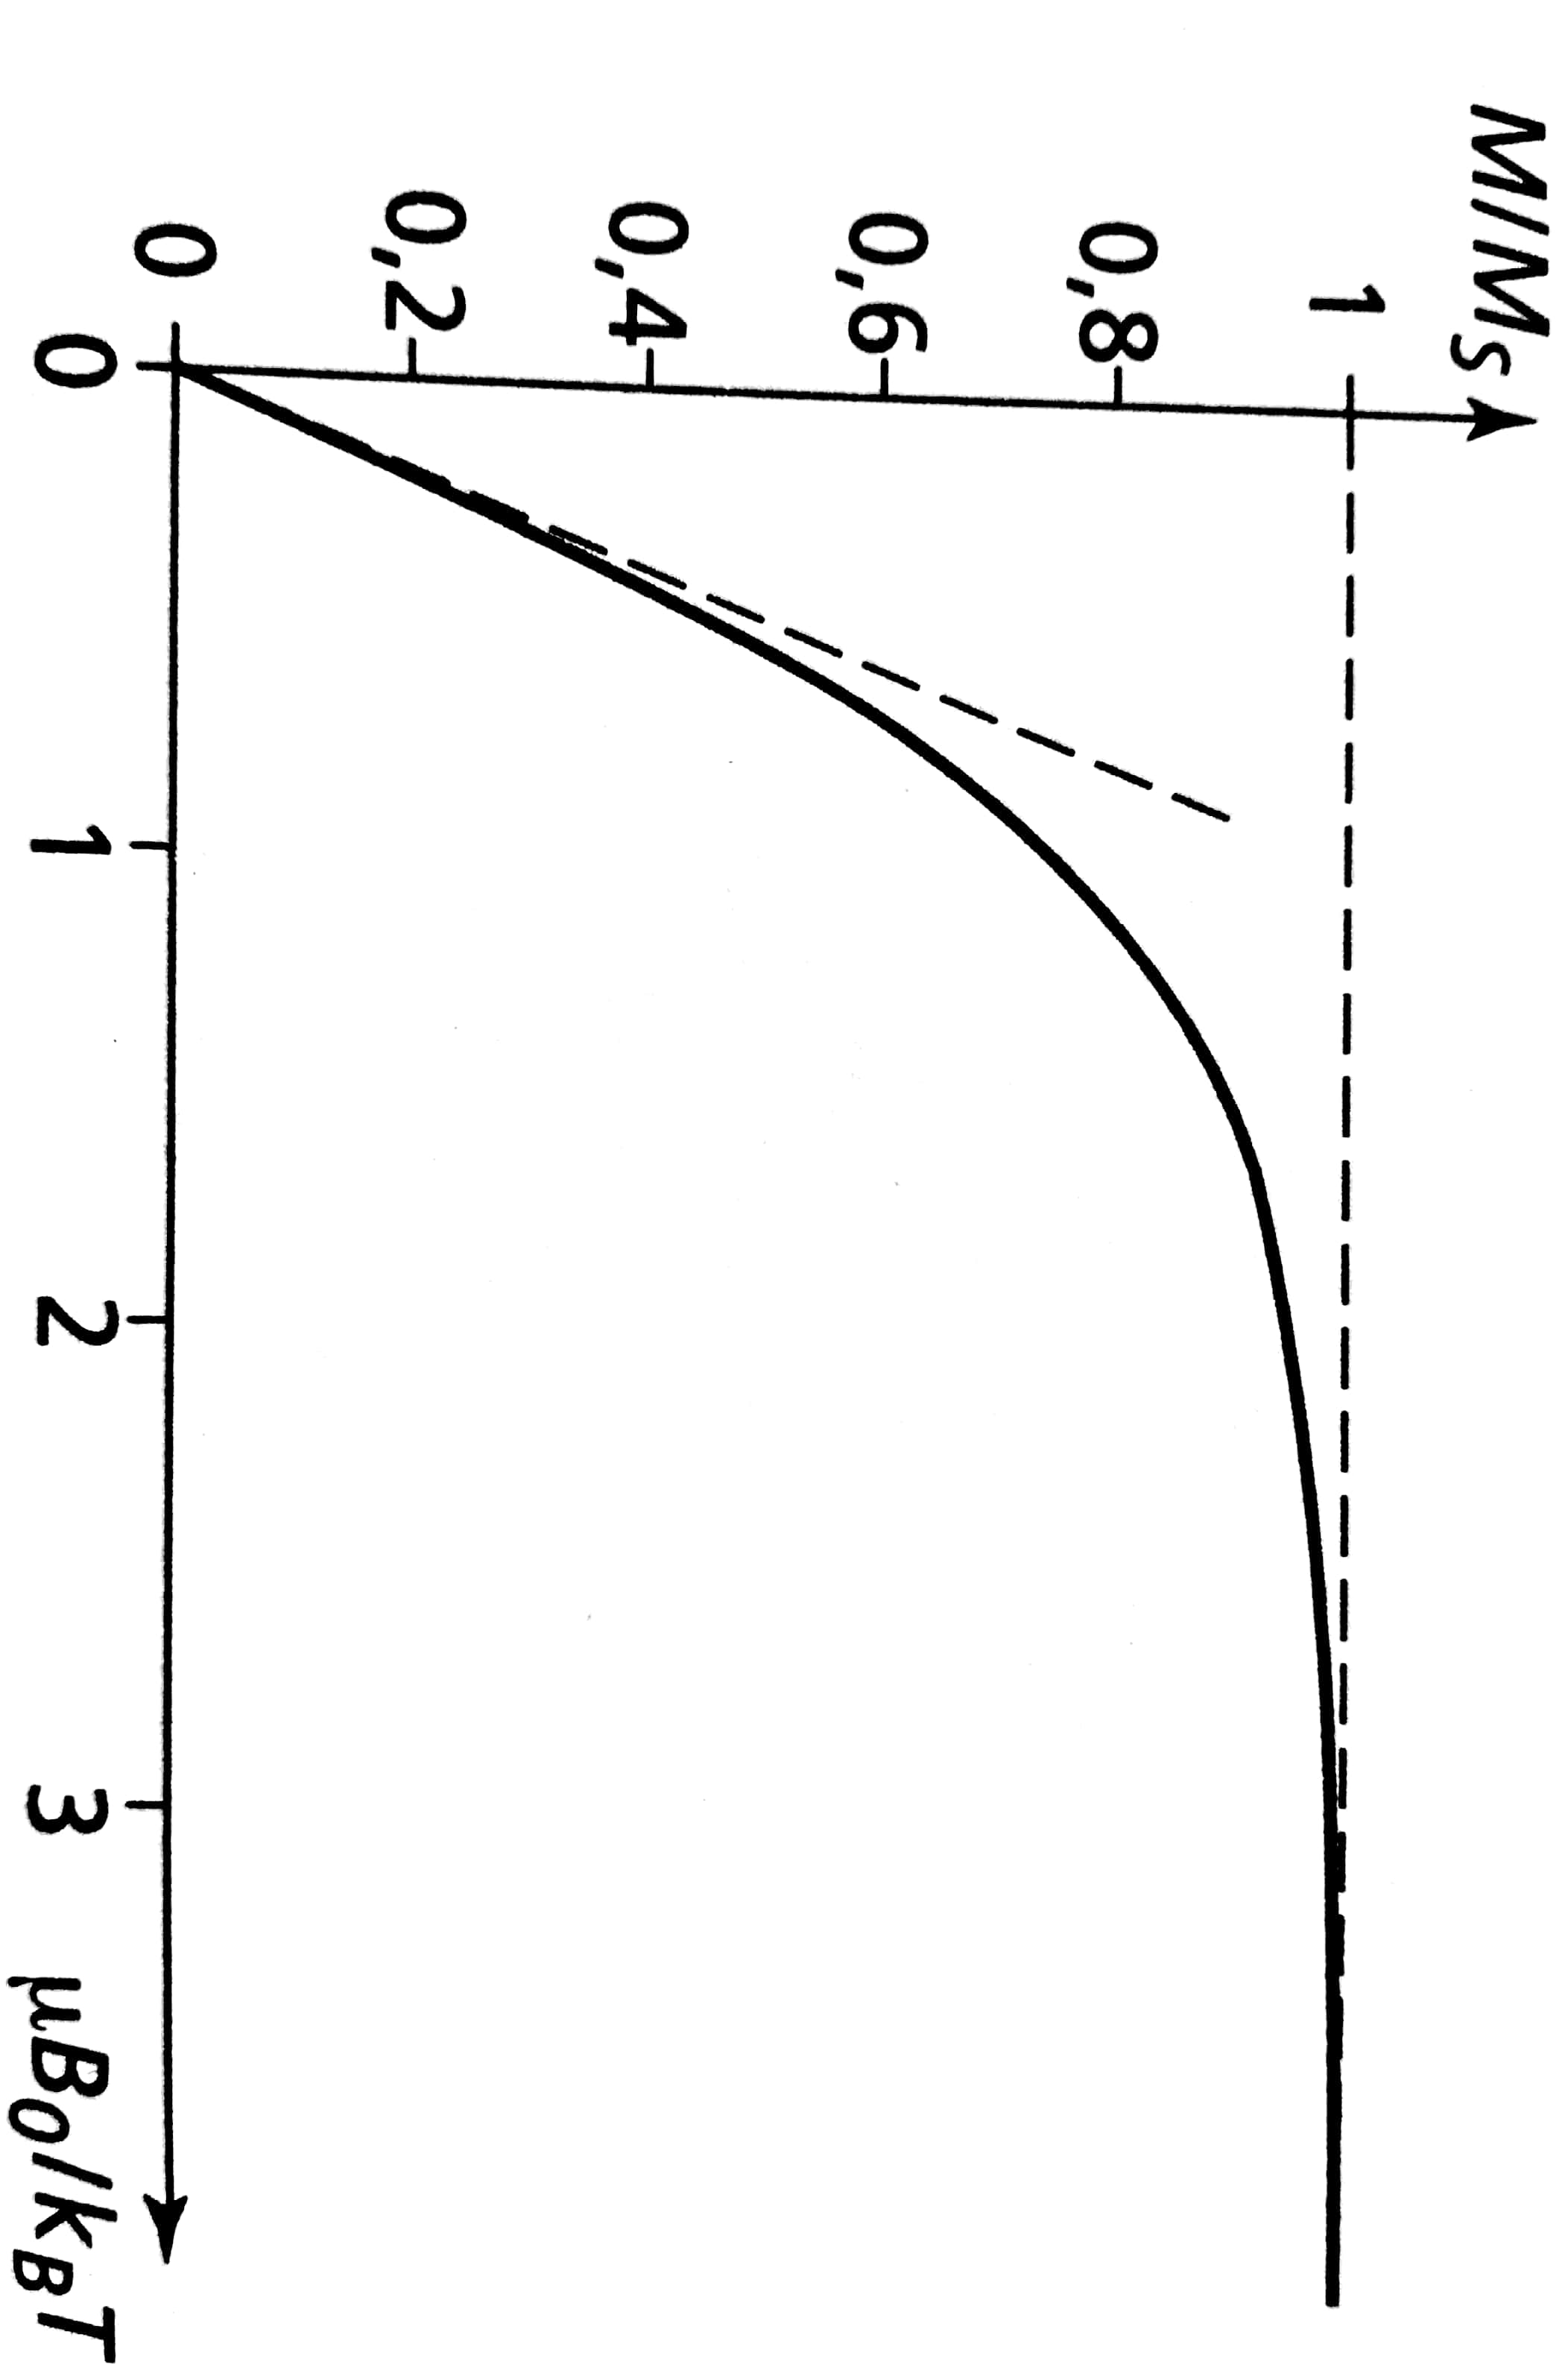
\includegraphics[width=5cm,angle=90]{para}
				\includegraphics[width=10cm]{cas_j_n0,5}}
				
\end{figure}

On voit qu'à très basse température ou a champ fort l'aimantation sature à la valeur $M_s$. Pour des températures telles que la température ambiante avec des champs raisonnables, l'argument de la tangente hyperbolique est petit devant un et on peut alors linéariser, au quel cas on constate qu'on a une relation du type $M = \chi_sB$ où $\chi$ est la susceptibilité, dans la pratique on utilisera la susceptibilité paramétrique $\chi_m= \mu_0\chi$ alors sans unité avec $\mu_0$ la perméabilité diélectrique du vide. Ici on a alors 
\begin{eqnarray}
\chi_m = \frac{1}{4k_BT}\mu_0 N(g\mu_B)^2
\end{eqnarray}
on a donc une variation en $1/T$ conforme avec les résultats expérimentaux : c'est la loi de Curie.\\

Le modèle que l'on vient d'expliciter permet de rendre compte des observations pour les matériaux dits paramagnétiques, mais il existe une autre classe de matériaux magnétiques possédant un comportement différent. En effet si on regarde le cas d'un aimant, les atomes qui le composent ont bien une activité magnétique, mais contrairement au cas explicité ici, ils ont une aimantation non nulle même en absence de champs extérieur ... pourquoi ? Sans doute dans ce cas ne peut on négliger l'interaction entre les moments magnétiques des atomes, tout simplement.

\section{Ferromagnétisme}
\textit{Complément III.J p445 du Diu de stat}\\
Pour introduire la notion regarder \textit{Magnétisme I de E du Trémolet p92}
\subsection{Présentation du phénomène}
On observe, pour les matériaux ferromagnétiques certaines propriétés intéressantes : si on place un aimant à coté d'un clou en fer, ce dernier est attiré vers l'aimant... mais si chauffe le clou au delà de 770°C alors le phénomène cesse... au delà de cette température critique appelée température du Curie il semble donc que les propriétés magnétiques du fer changent, on va ici voir pourquoi.\\  

On peut avoir accès aux comportement de l'aimantation en fonction du champ imposé et tracer expérimentalement le graphe représenté sur la figure suivante.

On constate que l'on a un cycle d'hystérésis, commenter.
Au delà de la température de Curie ce cycle disparait pour laisser place à une courbe similaire au cas des matériaux paramagnétiques.\\ 
\begin{figure}[h]
	\centerline{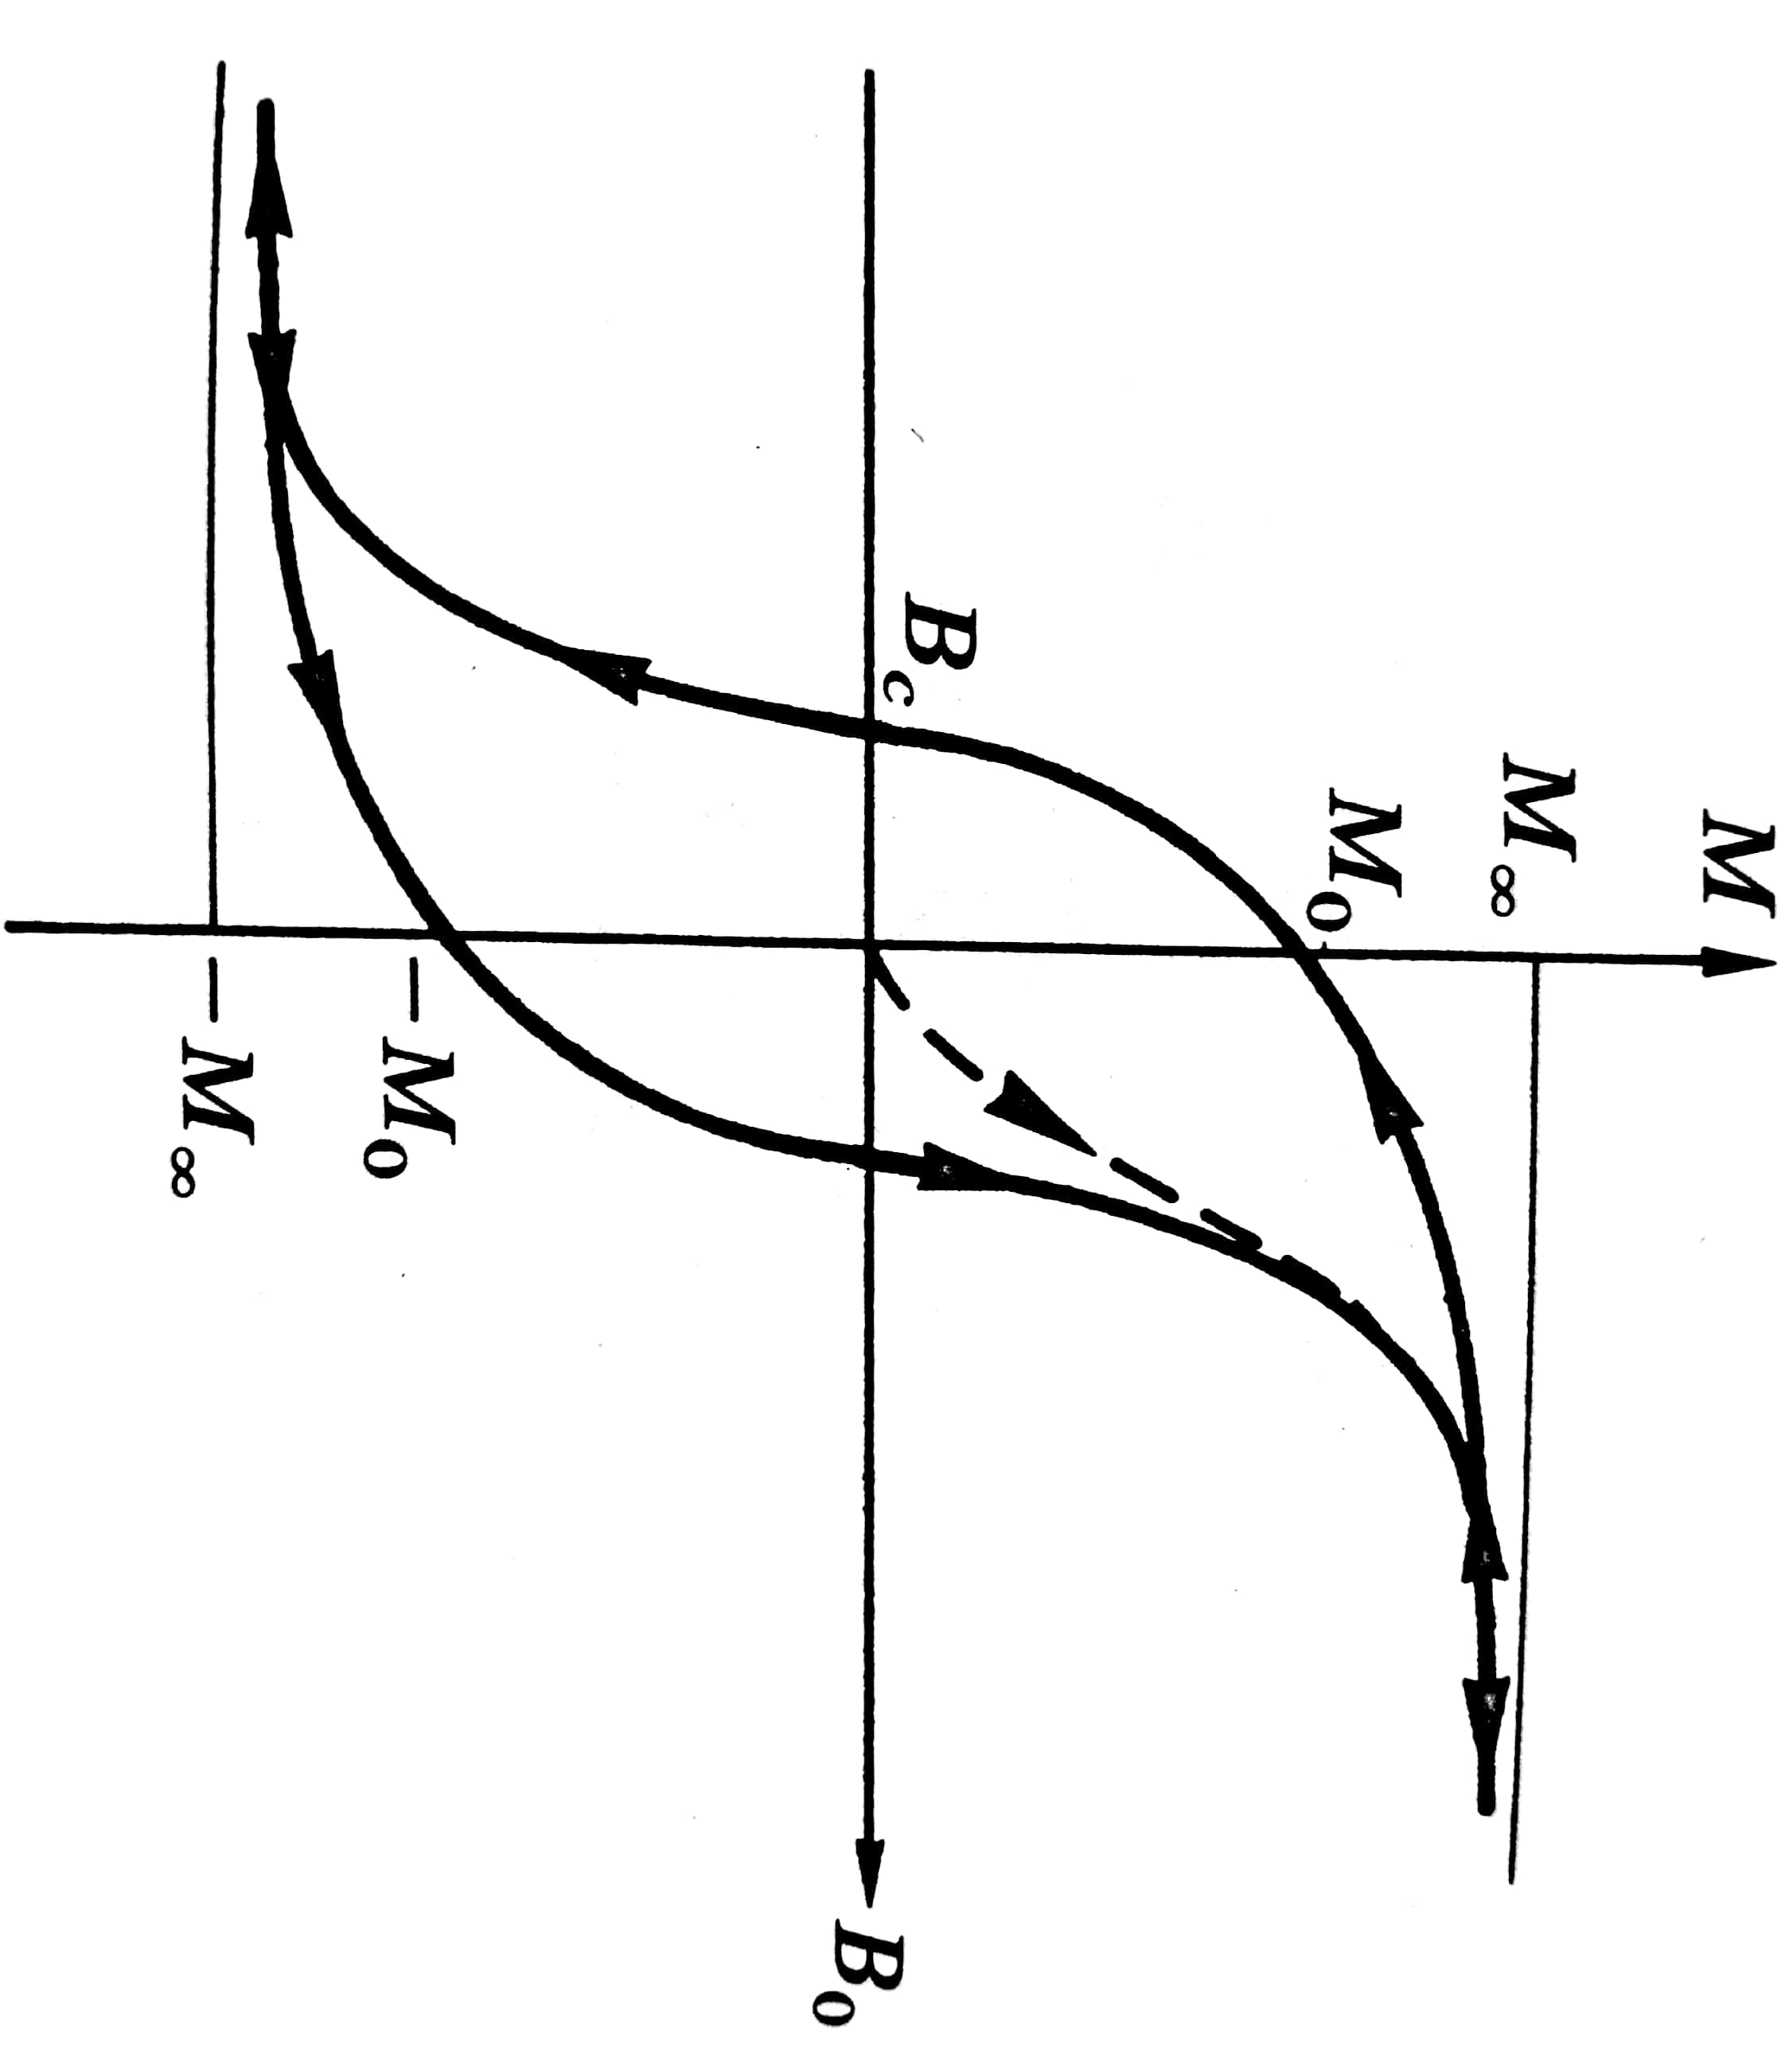
\includegraphics[width=7cm, angle=90]{hysteresis}
				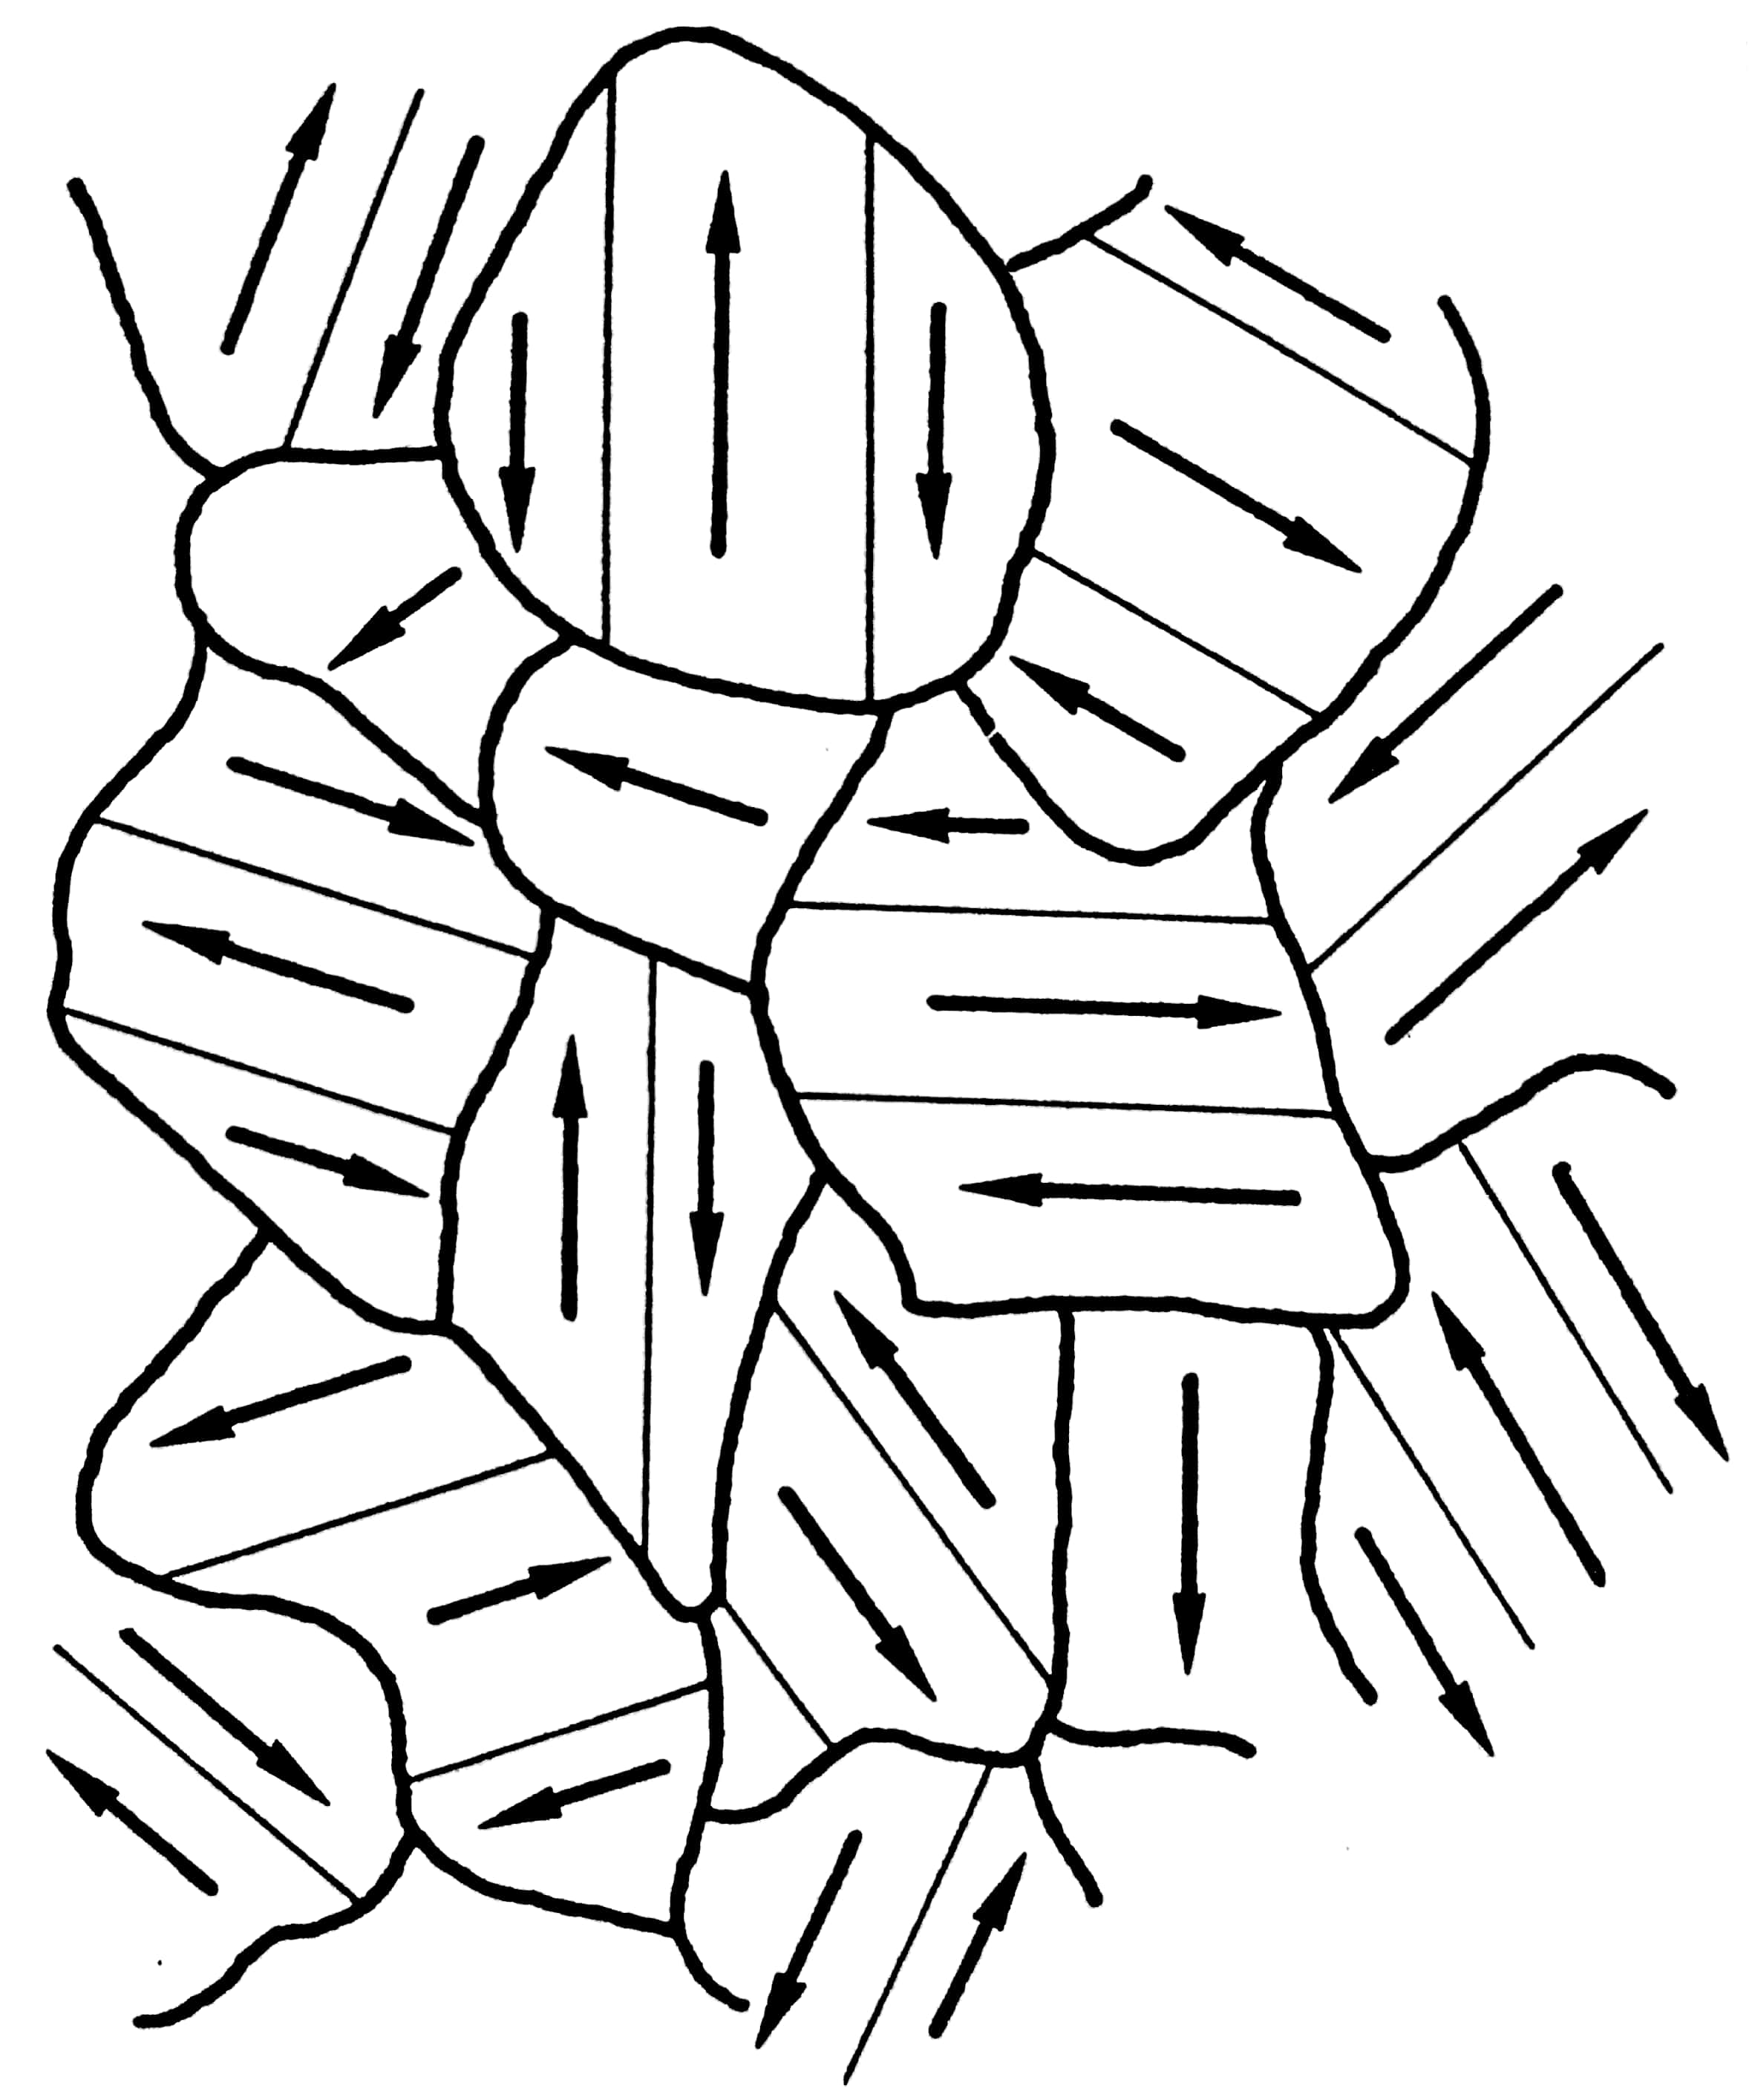
\includegraphics[width=7cm,angle=90]{weiss}}
\end{figure}

Pour expliquer ce comportement on va commencer par accepter l'hypothèse de Weiss, aujourd'hui vérifiée par microscopie, qui stipule qu'un cristal ferromagnétique est structuré en domaines possédant une aimantation non nulle mais ayant une orientation différente d'un domaine à l'autre. L'aimantation de ces domaines va alors s'aligner au champ extérieur au travers de deux dynamique distinctes : les domaines dont l'aimantation est alignée au champ grossissent, et l'aimantation des autres s'aligne selon le champ.\\

Maintenant qu'on a une idée qualitative de ce qui caractérise le ferromagnétisme on va regarder ce qu'il se passe plus en détail, en se plaçant dans un volume ne couvrant qu'un seul domaine de Weiss pour plus de simplicité.

\subsection{Étude quantitative}
On considère donc ici un cristal monoatomique de volume V en équilibre avec un thermostat à la température T et soumis à un champ magnétique uniforme $\vec{B} = B\vec{e}_z$. Les paramètres extérieurs sont donc $V$, $T$, et $\vec{B}$, et on cherche à déterminer l'expression de l'aimantation ou moment magnétique par unité de volume 
\begin{eqnarray}
\vec{M} = \frac{\vec{m}}{V}
\end{eqnarray}
en fonction de ces paramètre. Si on considère qu'il y a N spin $1/2$ dans ce volume V on a alors à priori 
\begin{eqnarray}
M = M_z  = \frac{Ng\mu_B}{2V} \mathrm{tanh}\left(\frac{g\mu_B B}{2k_BT}\right)
\end{eqnarray}
comme on l'a montré pour un solide paramagnétique dans lequel les spins n'interagissent pas entre eux. Mais dans ce cas $M$ s'annule à champ nul et ce quel que soit la température, ce qui n'est pas en accord avec les observations. Il faut donc cette fois prendre en compte les interaction spin-spin, que l'on peut à priori modéliser de façon générale par l'énergie d'interaction 
\begin{eqnarray}
H_{ij} = -J_{ij}\vec{S}_i.\vec{S}_j,
\end{eqnarray}
où $J_{ij}$ doit être positif pour que les spin s'alignent, et ne peut que décroitre avec la distance entre les atomes. Par conséquent on peut raisonnablement considérer le cas simple où seuls les premiers voisins interagissent, ce qui mène au hamiltonien total pour le cristal 
\begin{eqnarray}
\mathcal{H} = -g\mu_B \vec{B}.\sum_{i=1}^N \vec{S}_i \;-\; \;J\sum_{premiers\;voisins} \vec{S}_i.\vec{S}_j
\end{eqnarray}
appelé hamiltonien de Heisenberg. Ce hamiltonien est la somme de nombreux termes couplés et on est pas capable, à ce jour, d'en déduire analytiquement la fonction de partition associée, on va tout de même pouvoir obtenir un résultat en faisant une approximation de champs moyen.

\subsection{Approximation de champ moyen}
C'est une approximation courante en physique du solide qui consiste, dans un problème où on considère l'interaction d'un corps avec un grand nombre d'autres éléments décorrélés, à considérer que cette interaction peut se résumer à une interaction avec un champ moyen représentant l'ensemble des autres corps.\\

On a, pour un site $i$ du réseau,
\begin{eqnarray}
H_i = -\vec{S}_i . [g\mu_B \vec{B} + J \sum_{j\in v(i)}\vec{S}_j]
\end{eqnarray}
où $v(i)$ est l'ensemble des plus proches voisins du site $i$. On voit que tout se passe comme si ce site était soumis à un champ magnétique effectif 
\begin{eqnarray}
\vec{B}^{(i)} = \vec{B} + \frac{J}{g\mu_B}\sum_{j\in v(i)} \vec{S}_j\hspace{1cm}\Longrightarrow\hspace{1cm} H_i = -g\mu_B\vec{S}_i.\vec{B}^{(i)}
\end{eqnarray}
L'approximation de champ moyen consiste alors à négliger les fluctuations de ce champ effectif et à le remplacer par sa valeur moyenne. Or, dans un cristal chaque spin a la même valeur moyenne définie à partir de l'aimantation
\begin{eqnarray}
\langle\vec{S}_i\rangle = \frac{V}{Ng\mu_B}\vec{M}
\end{eqnarray} 
et on en déduit ainsi 
\begin{eqnarray}
\vec{B}_{eff} = \langle\vec{B}^{(i)}\rangle = \vec{B} + \lambda \vec{M} \hspace{1cm}\mathrm{avec}\hspace{1cm}\lambda = \frac{pJ}{(g\mu_B)^2}\frac{V}{N}
\end{eqnarray}
où p est le nombre de premier voisins. On voit alors que le champ effectif ne dépend plus du site : on a donc découplé le Hamiltonien de Heisenberg. De plus, le problème se ramène maintenant au cas du paramagnétisme mais avec cette fois un champ effectif, on a donc 
\begin{eqnarray}
M = N\frac{g\mu_B}{2V}\mathrm{tanh}\left(\frac{g\mu_B}{2kT}B_{eff}\right) =  N\frac{g\mu_B}{2V}\mathrm{tanh}\left(\frac{g\mu_B}{2kT}(B+\lambda M)\right)
\end{eqnarray}
(où on a projeté $\vec{B}$ et $\vec{M}$ sur $\vec{e}_z$ puisque à l'équilibre les deux sont alignés selon le même axe). On constate que cette fois le second membre dépend de l'aimantation, les solutions de cette équation vont donc nous donner les valeurs permises de l'aimantation. Cette équation est plus facile à résoudre graphiquement en regardant les intersections des deux fonctions de l'aimantation.

\section{Résolution, transition ferro-para}
\subsubsection{En champ nul}
On a 
\begin{eqnarray}
\frac{M}{M_{\infty}} = \mathrm{tanh}\left(\frac{pJ}{4k_BT}\frac{M}{M_{\infty}}\right) = \mathrm{tanh}\left(\frac{T_c}{T}\frac{M}{M_{\infty}}\right)
\hspace{2cm} M_{\infty} =\frac{Ng\mu_B}{2V} \label{M0}
\end{eqnarray}

\begin{figure}[h]
	\centerline{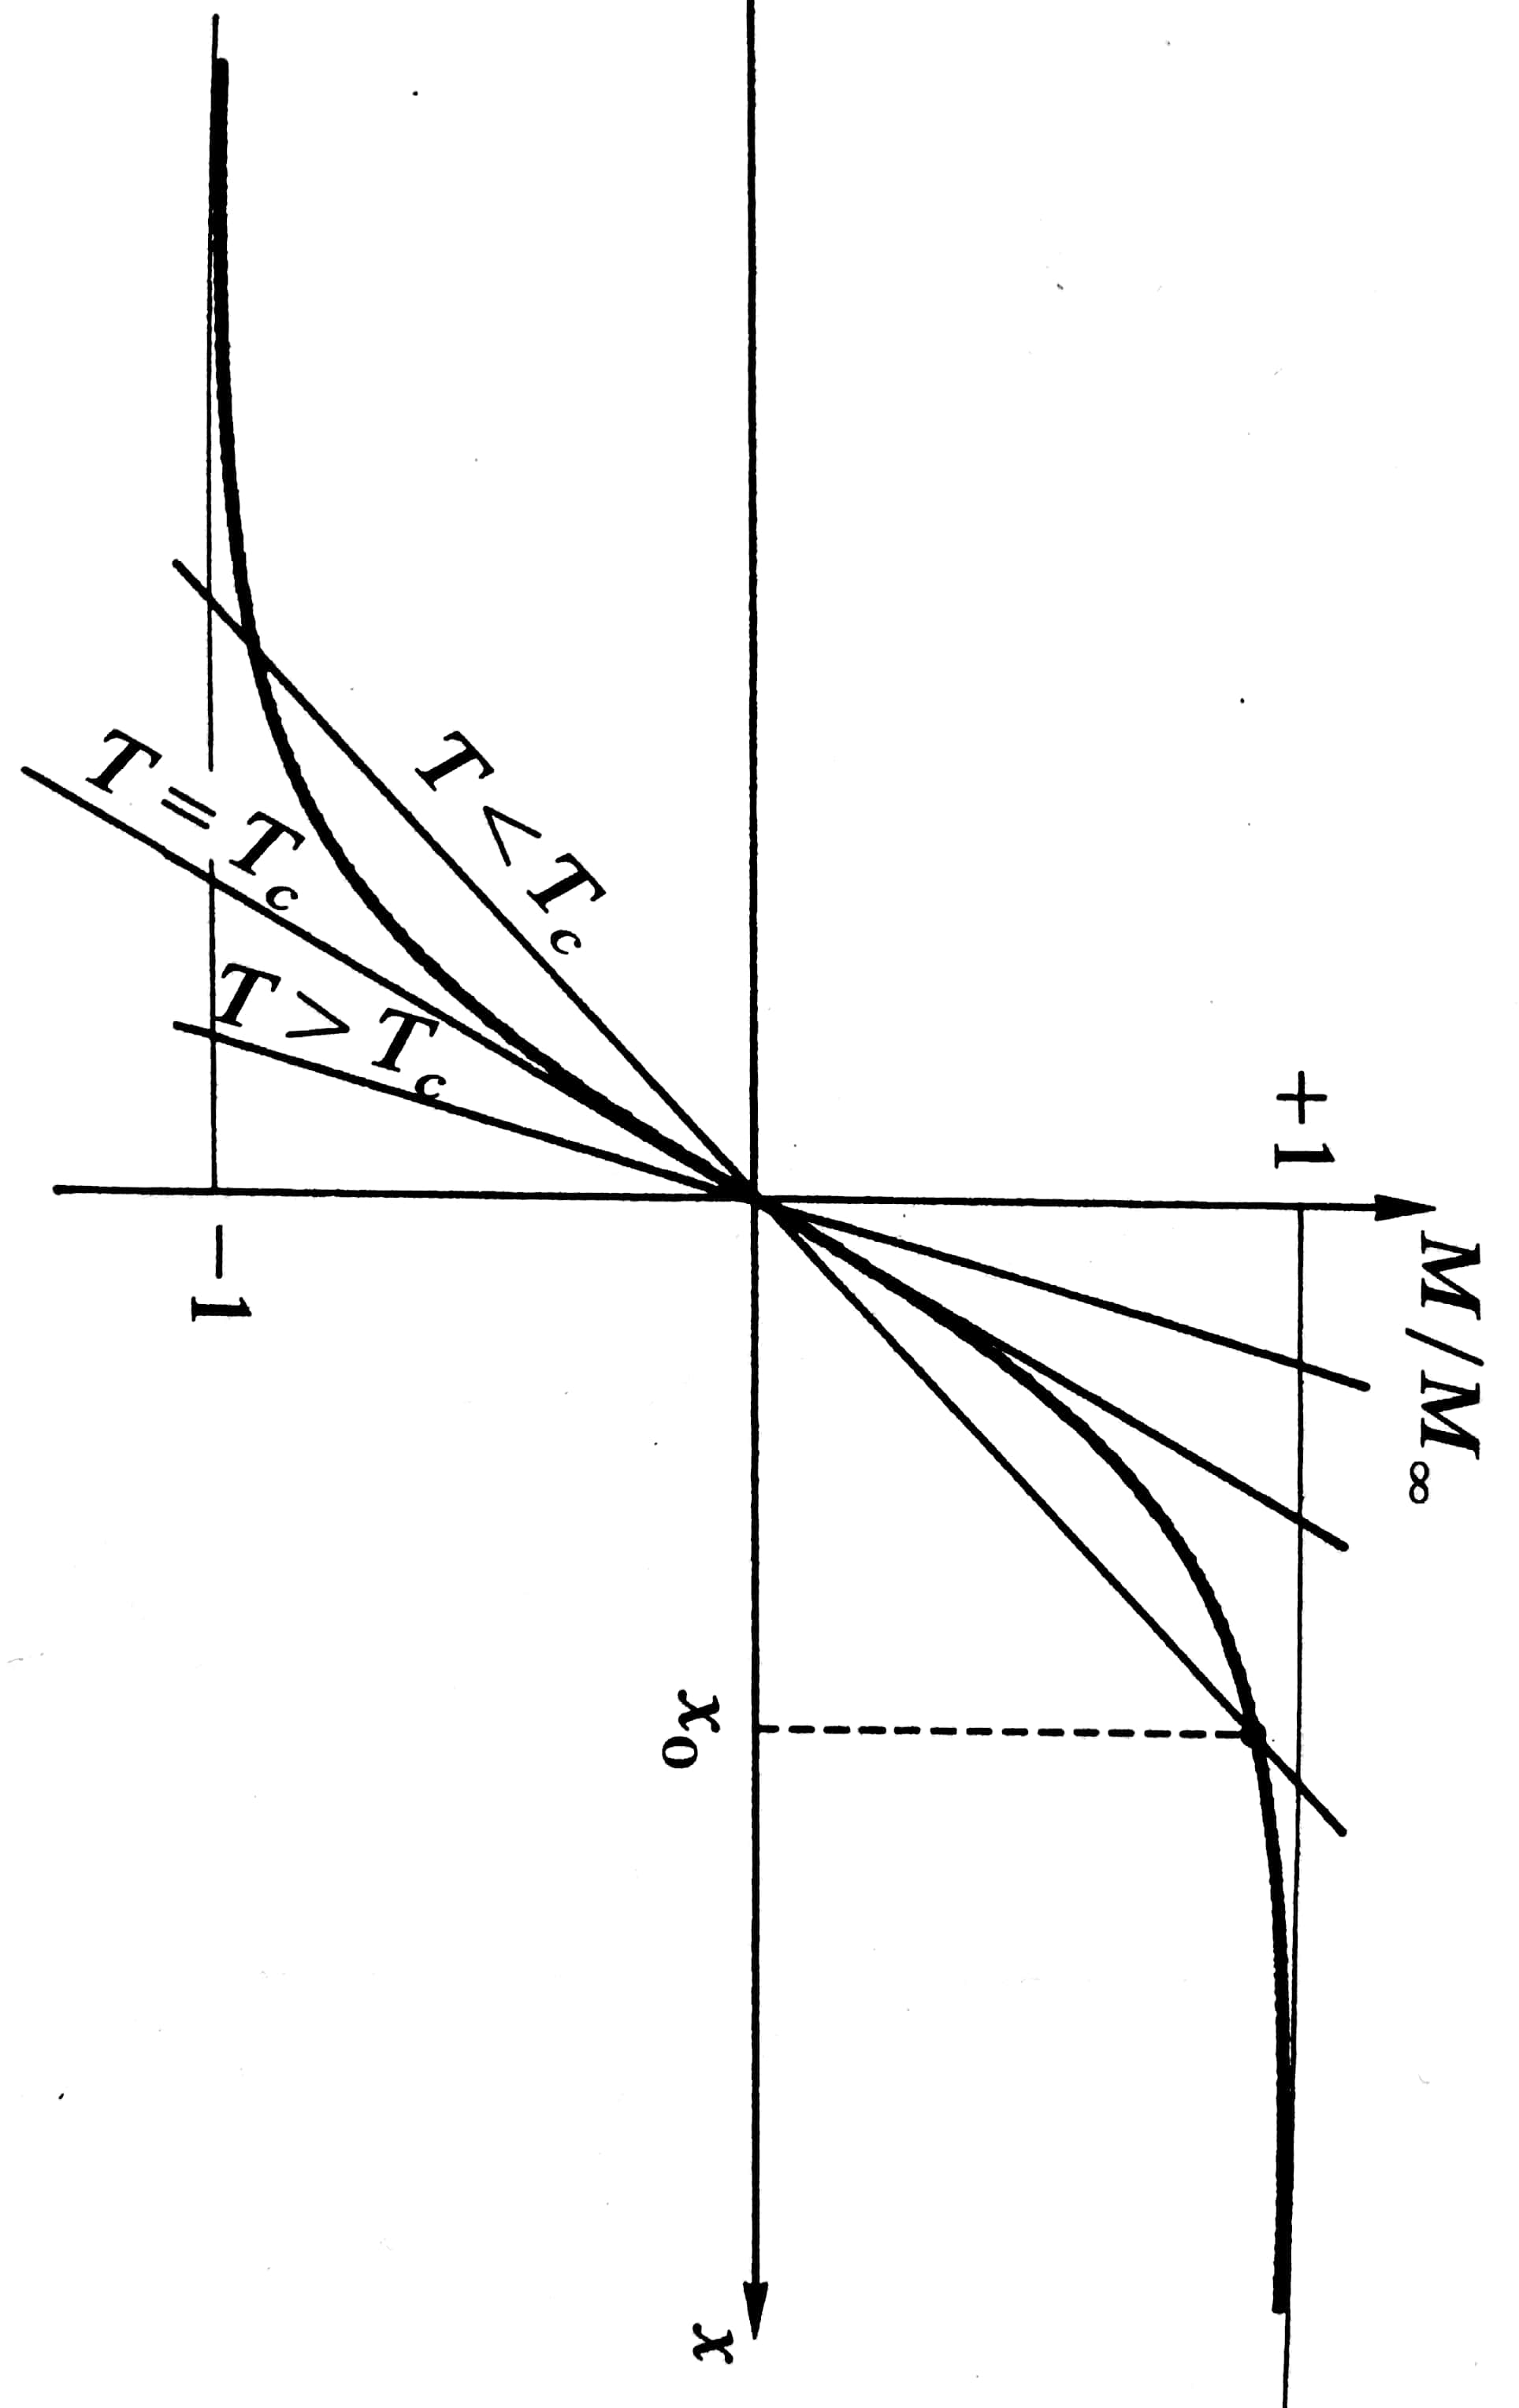
\includegraphics[width=5cm,angle=90]{Mx3}
		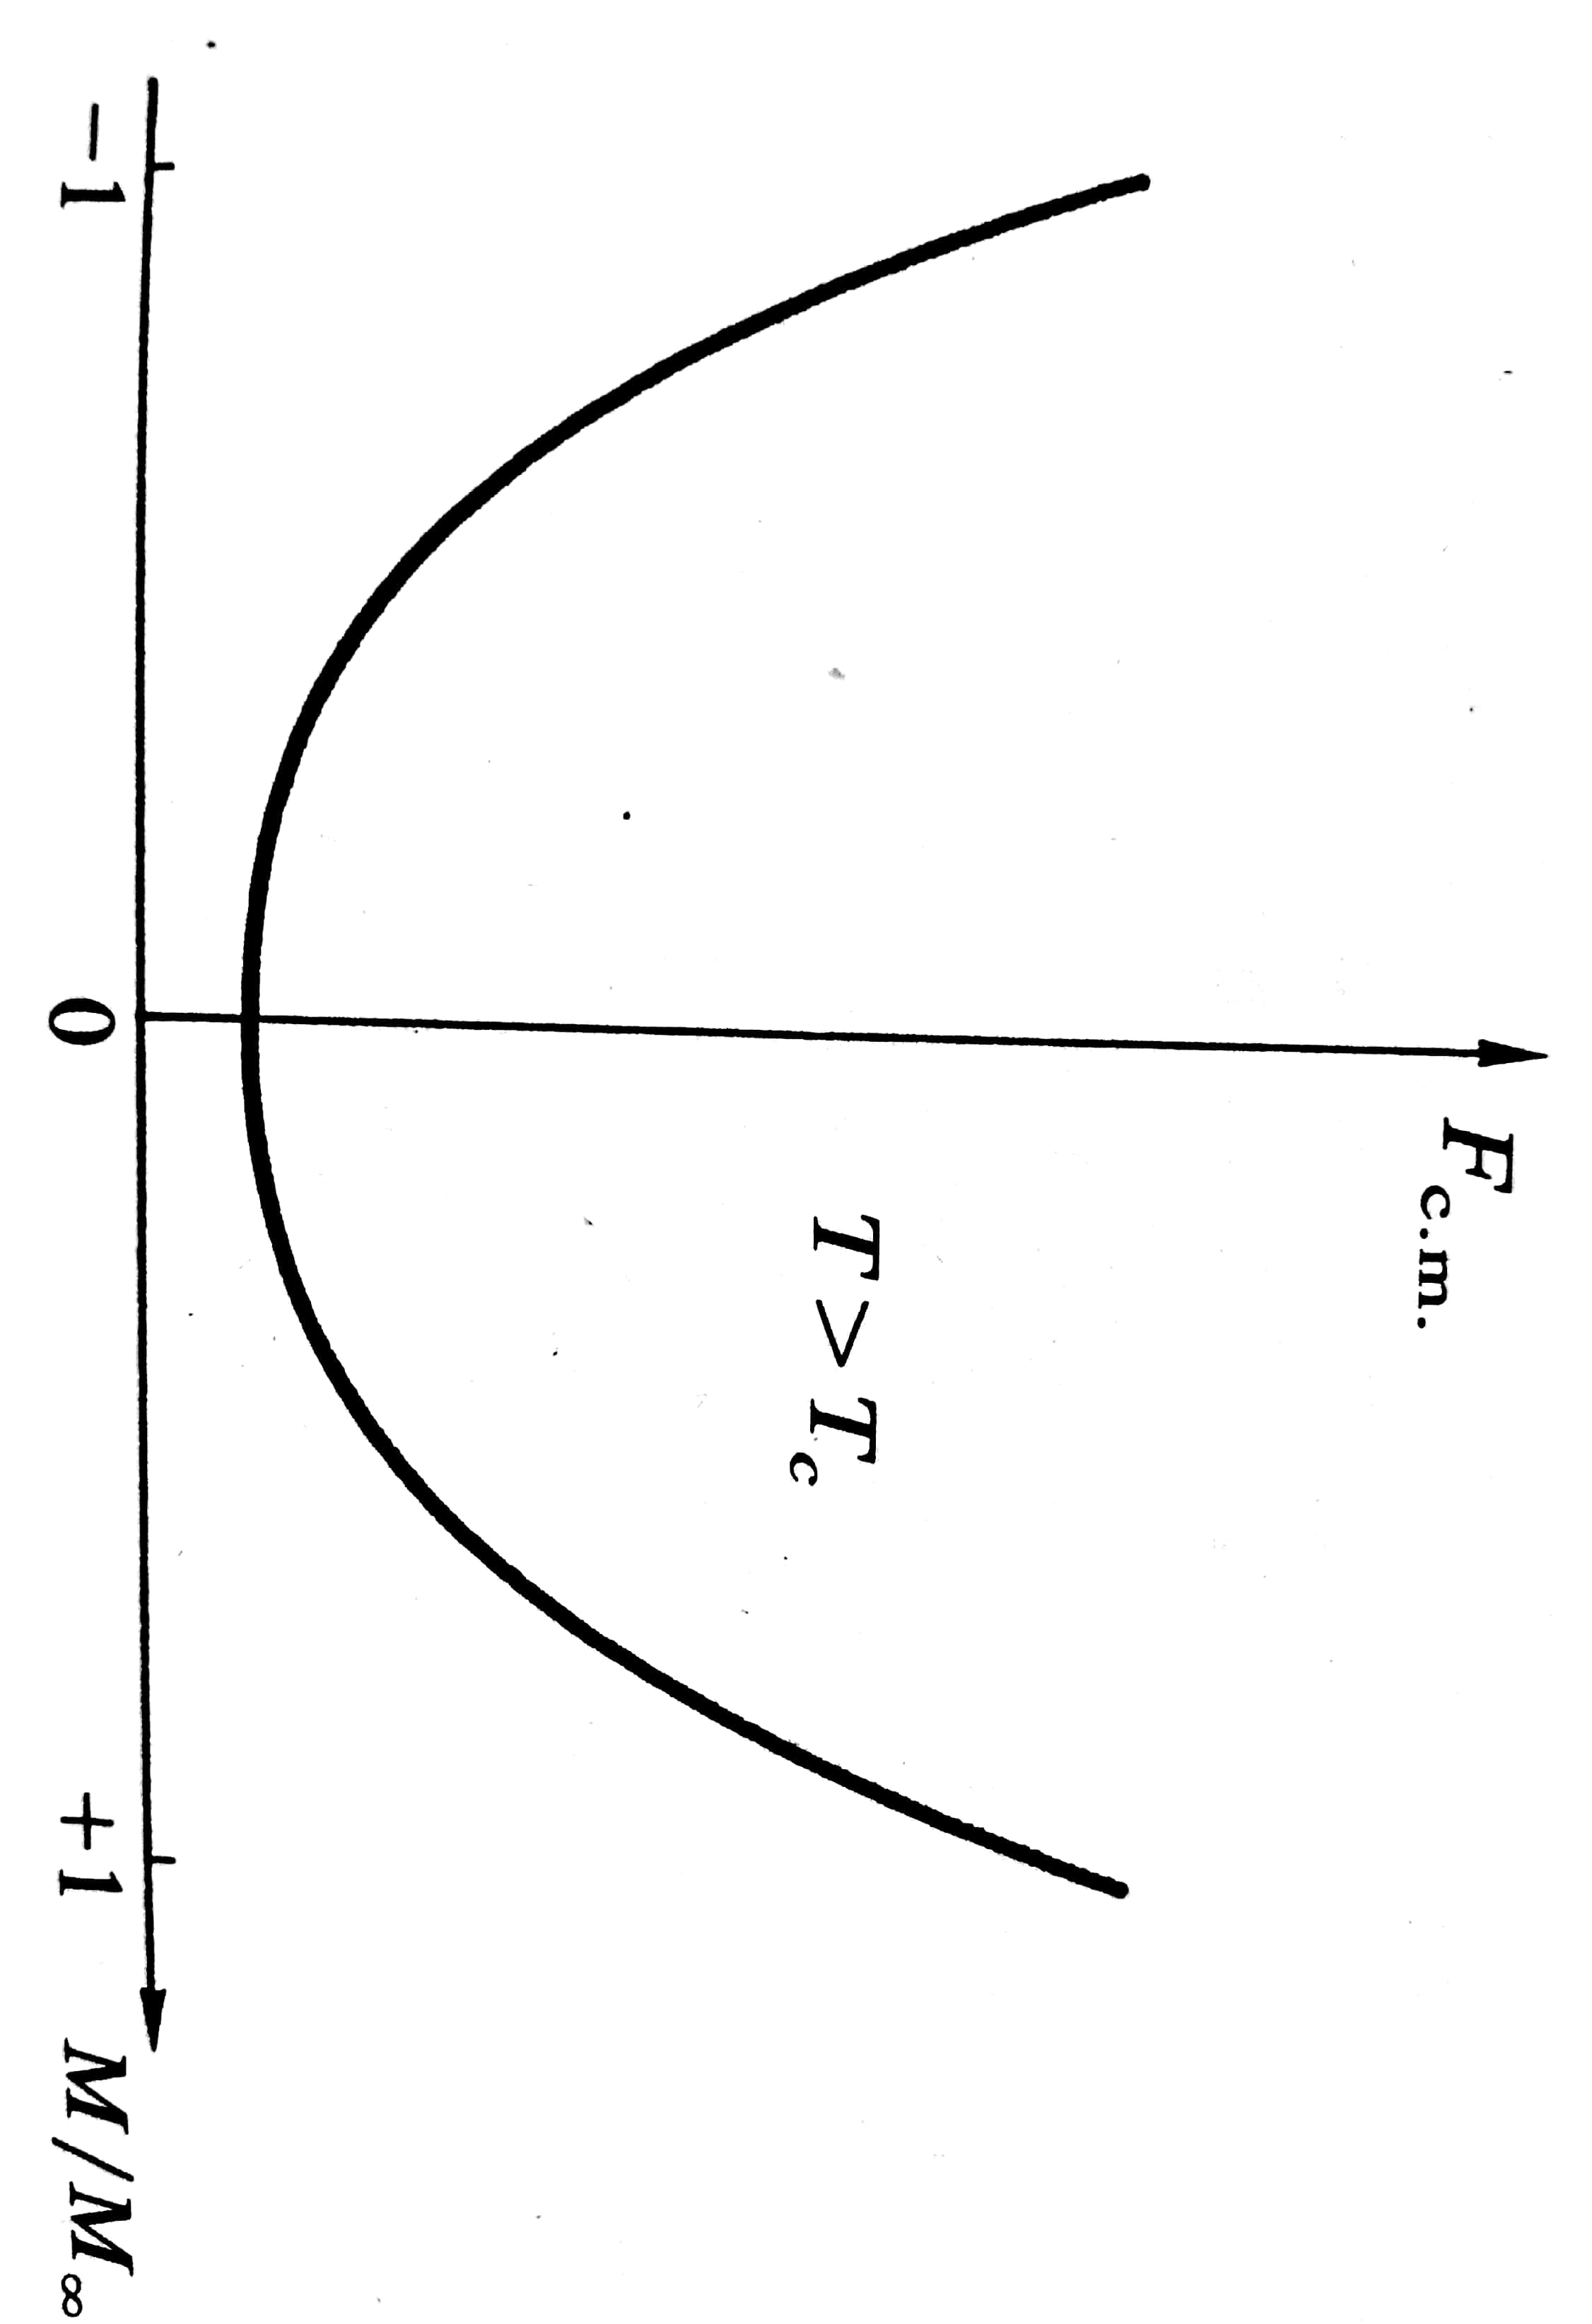
\includegraphics[width=4cm,angle=90]{F_T_sup_Tc}
		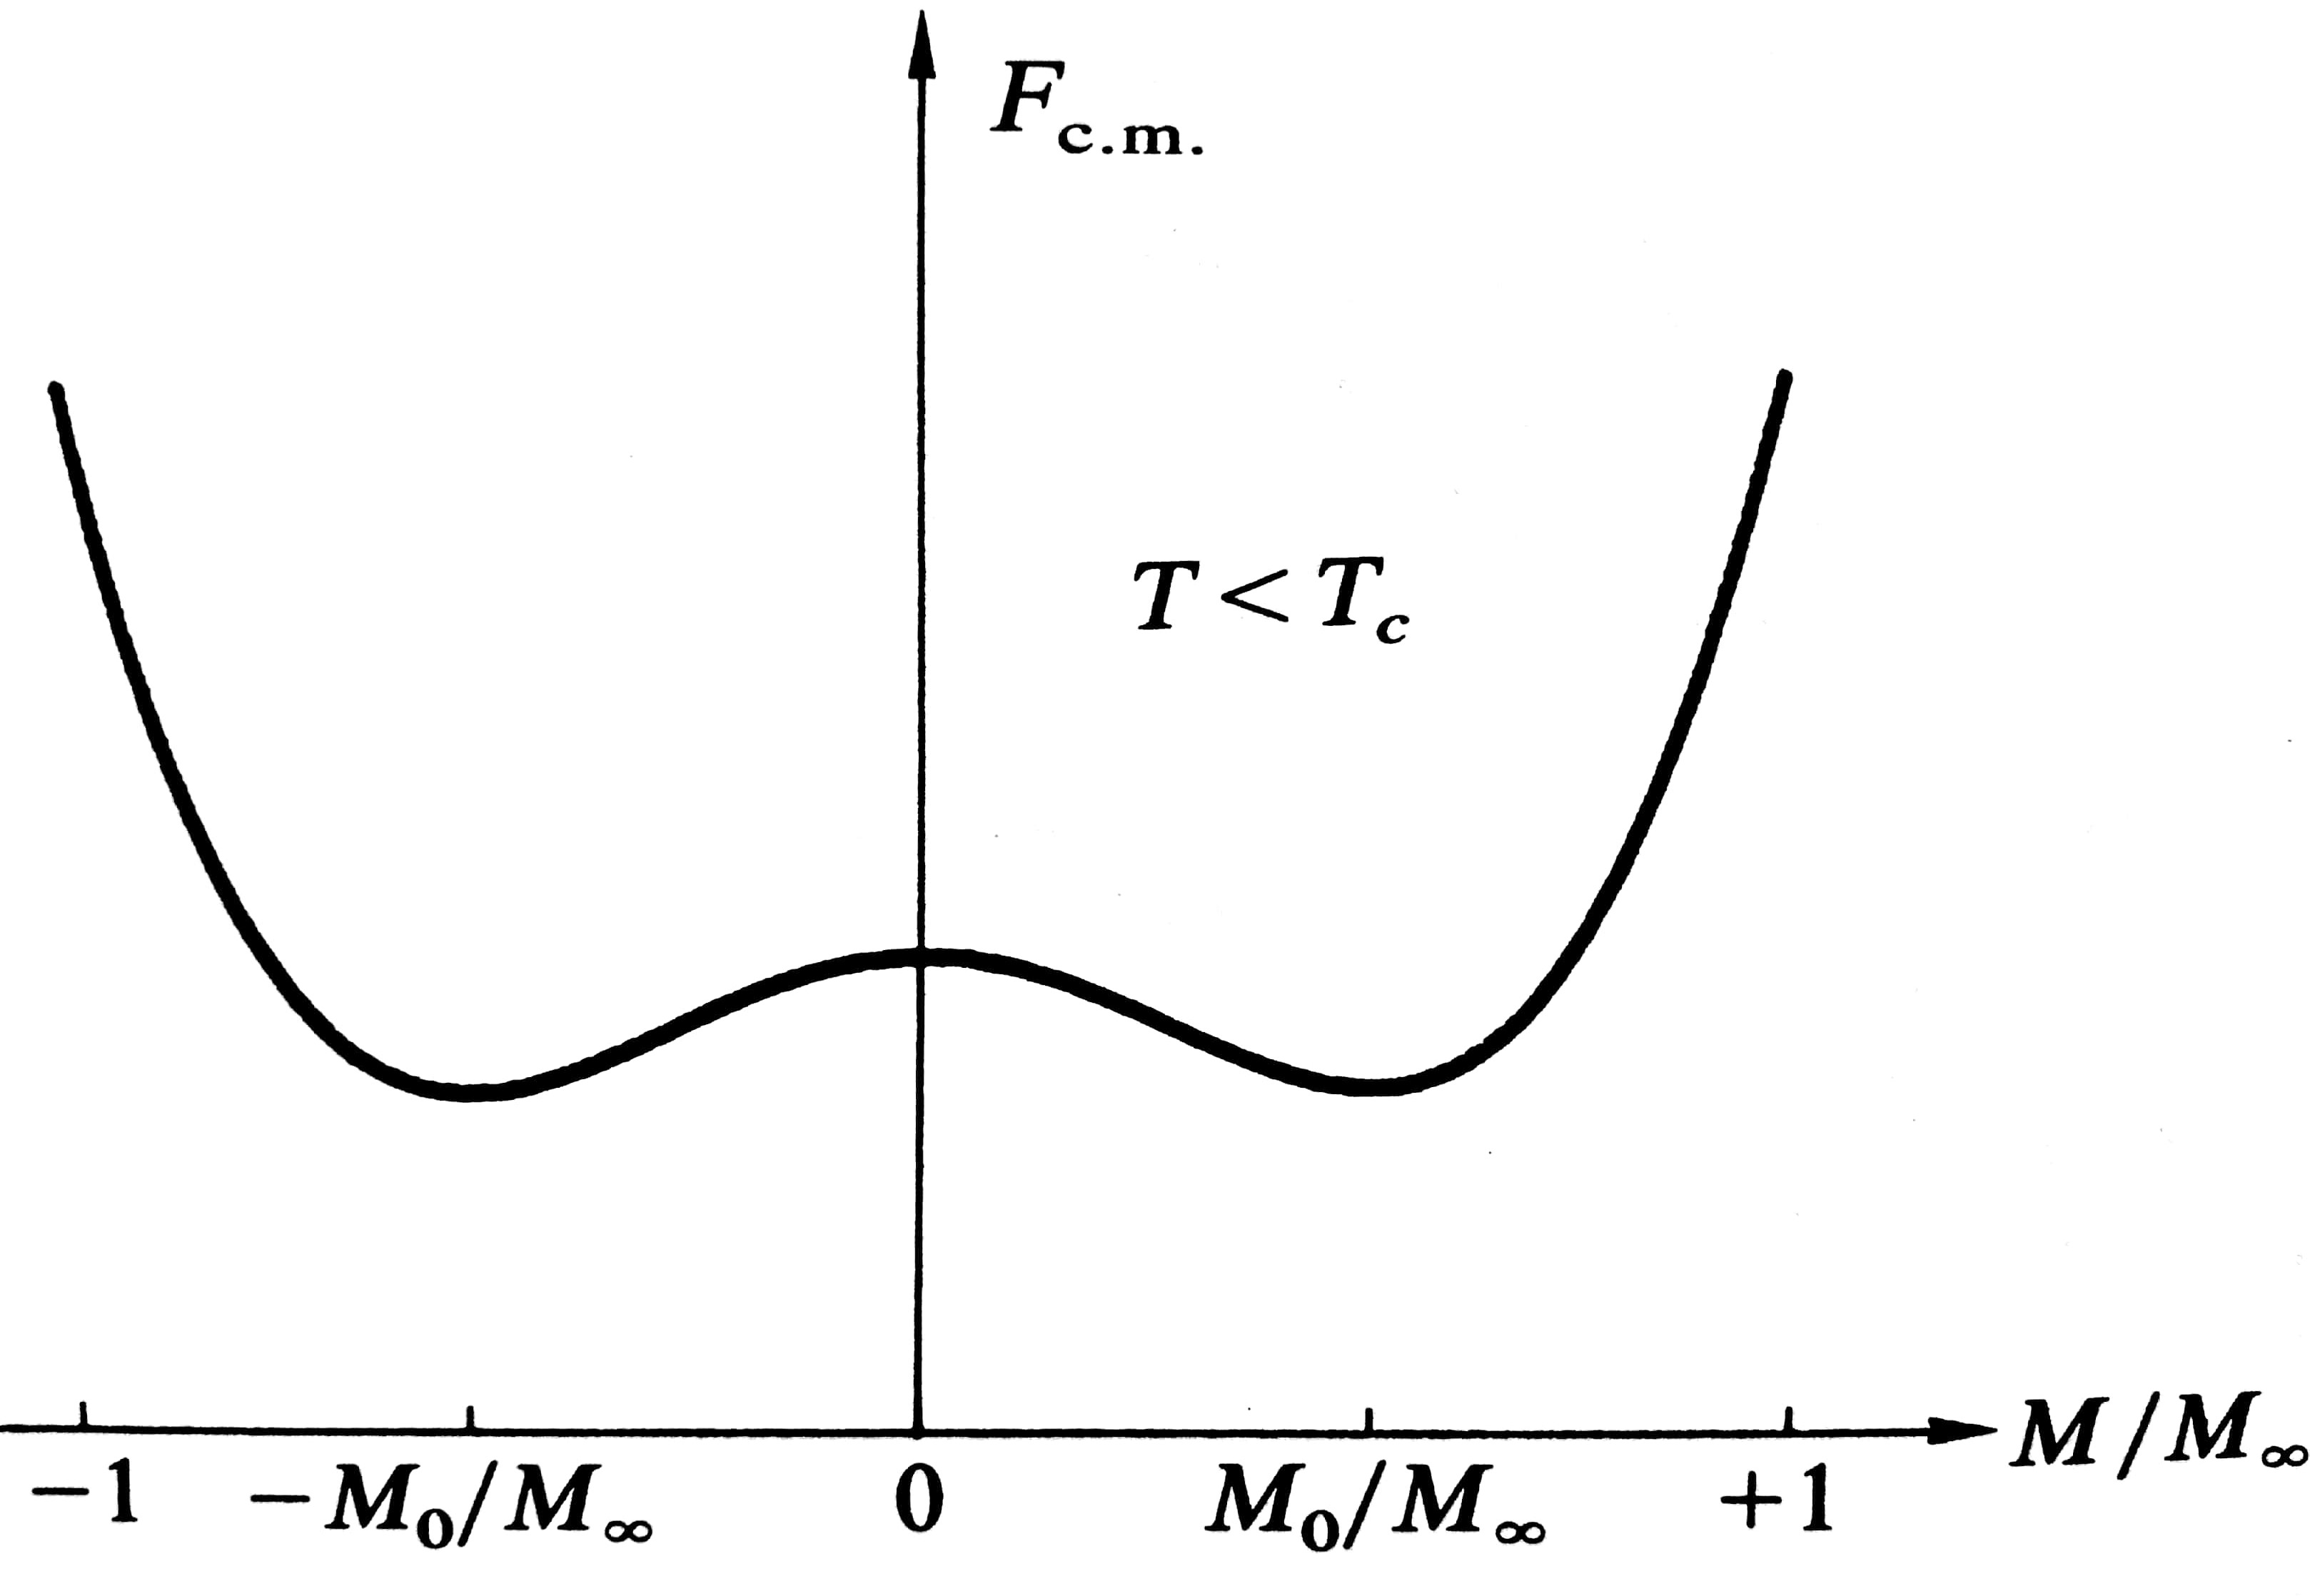
\includegraphics[width=5.5cm]{F_T_inf_Tc}}
\end{figure}

On peut facilement calculer l'énergie libre à partir du hamiltonien que l'on a établi, elle va nous permettre de voir si les solutions de (\ref{M0}) sont stables.

\subsubsection{Cas général}
Dans le cas général on a
\begin{eqnarray}
\frac{M}{M_{\infty}} = \mathrm{tanh}\left(\frac{T_c}{T}(B+\lambda M)\right) = \mathrm{tanh}\left(\frac{g\mu_BB}{2k_BT} + \frac{T_c}{T}\frac{M}{M_{\infty}}\right)
\end{eqnarray}
que l'on a représenté sur la figure suivante 
\begin{figure}[h]
	\centerline{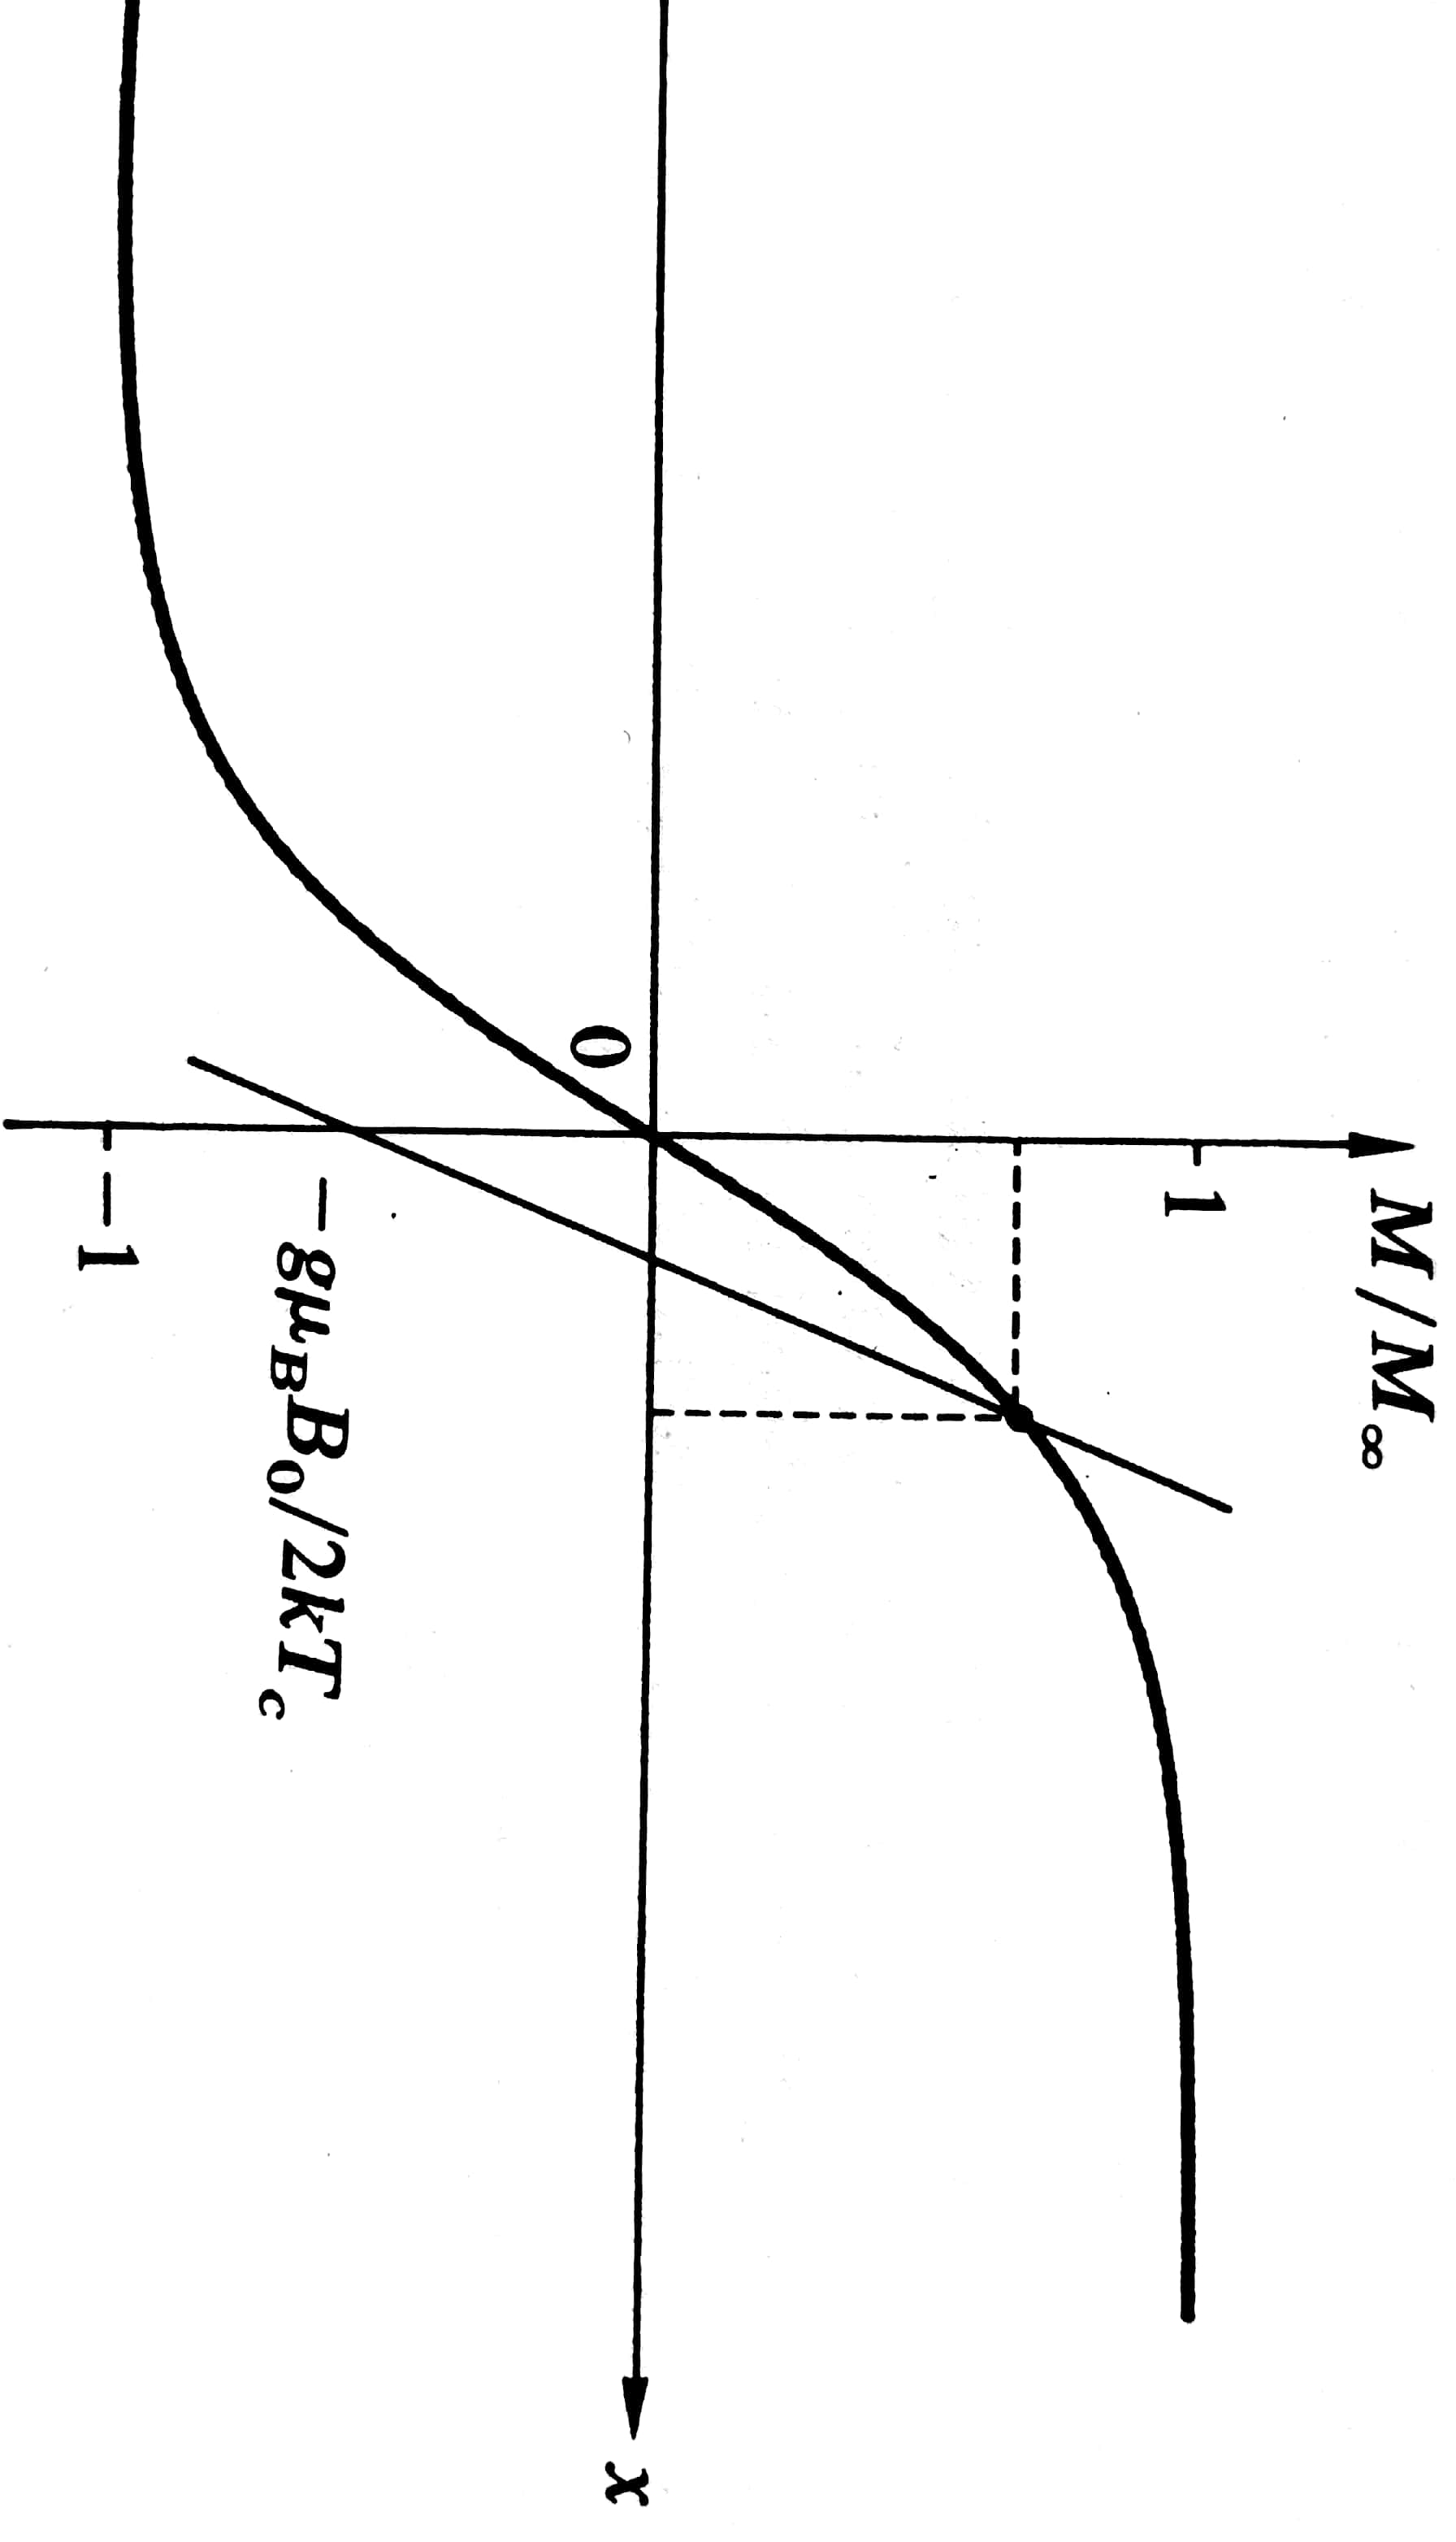
\includegraphics[width=3.8cm,angle=90]{Mx2}
		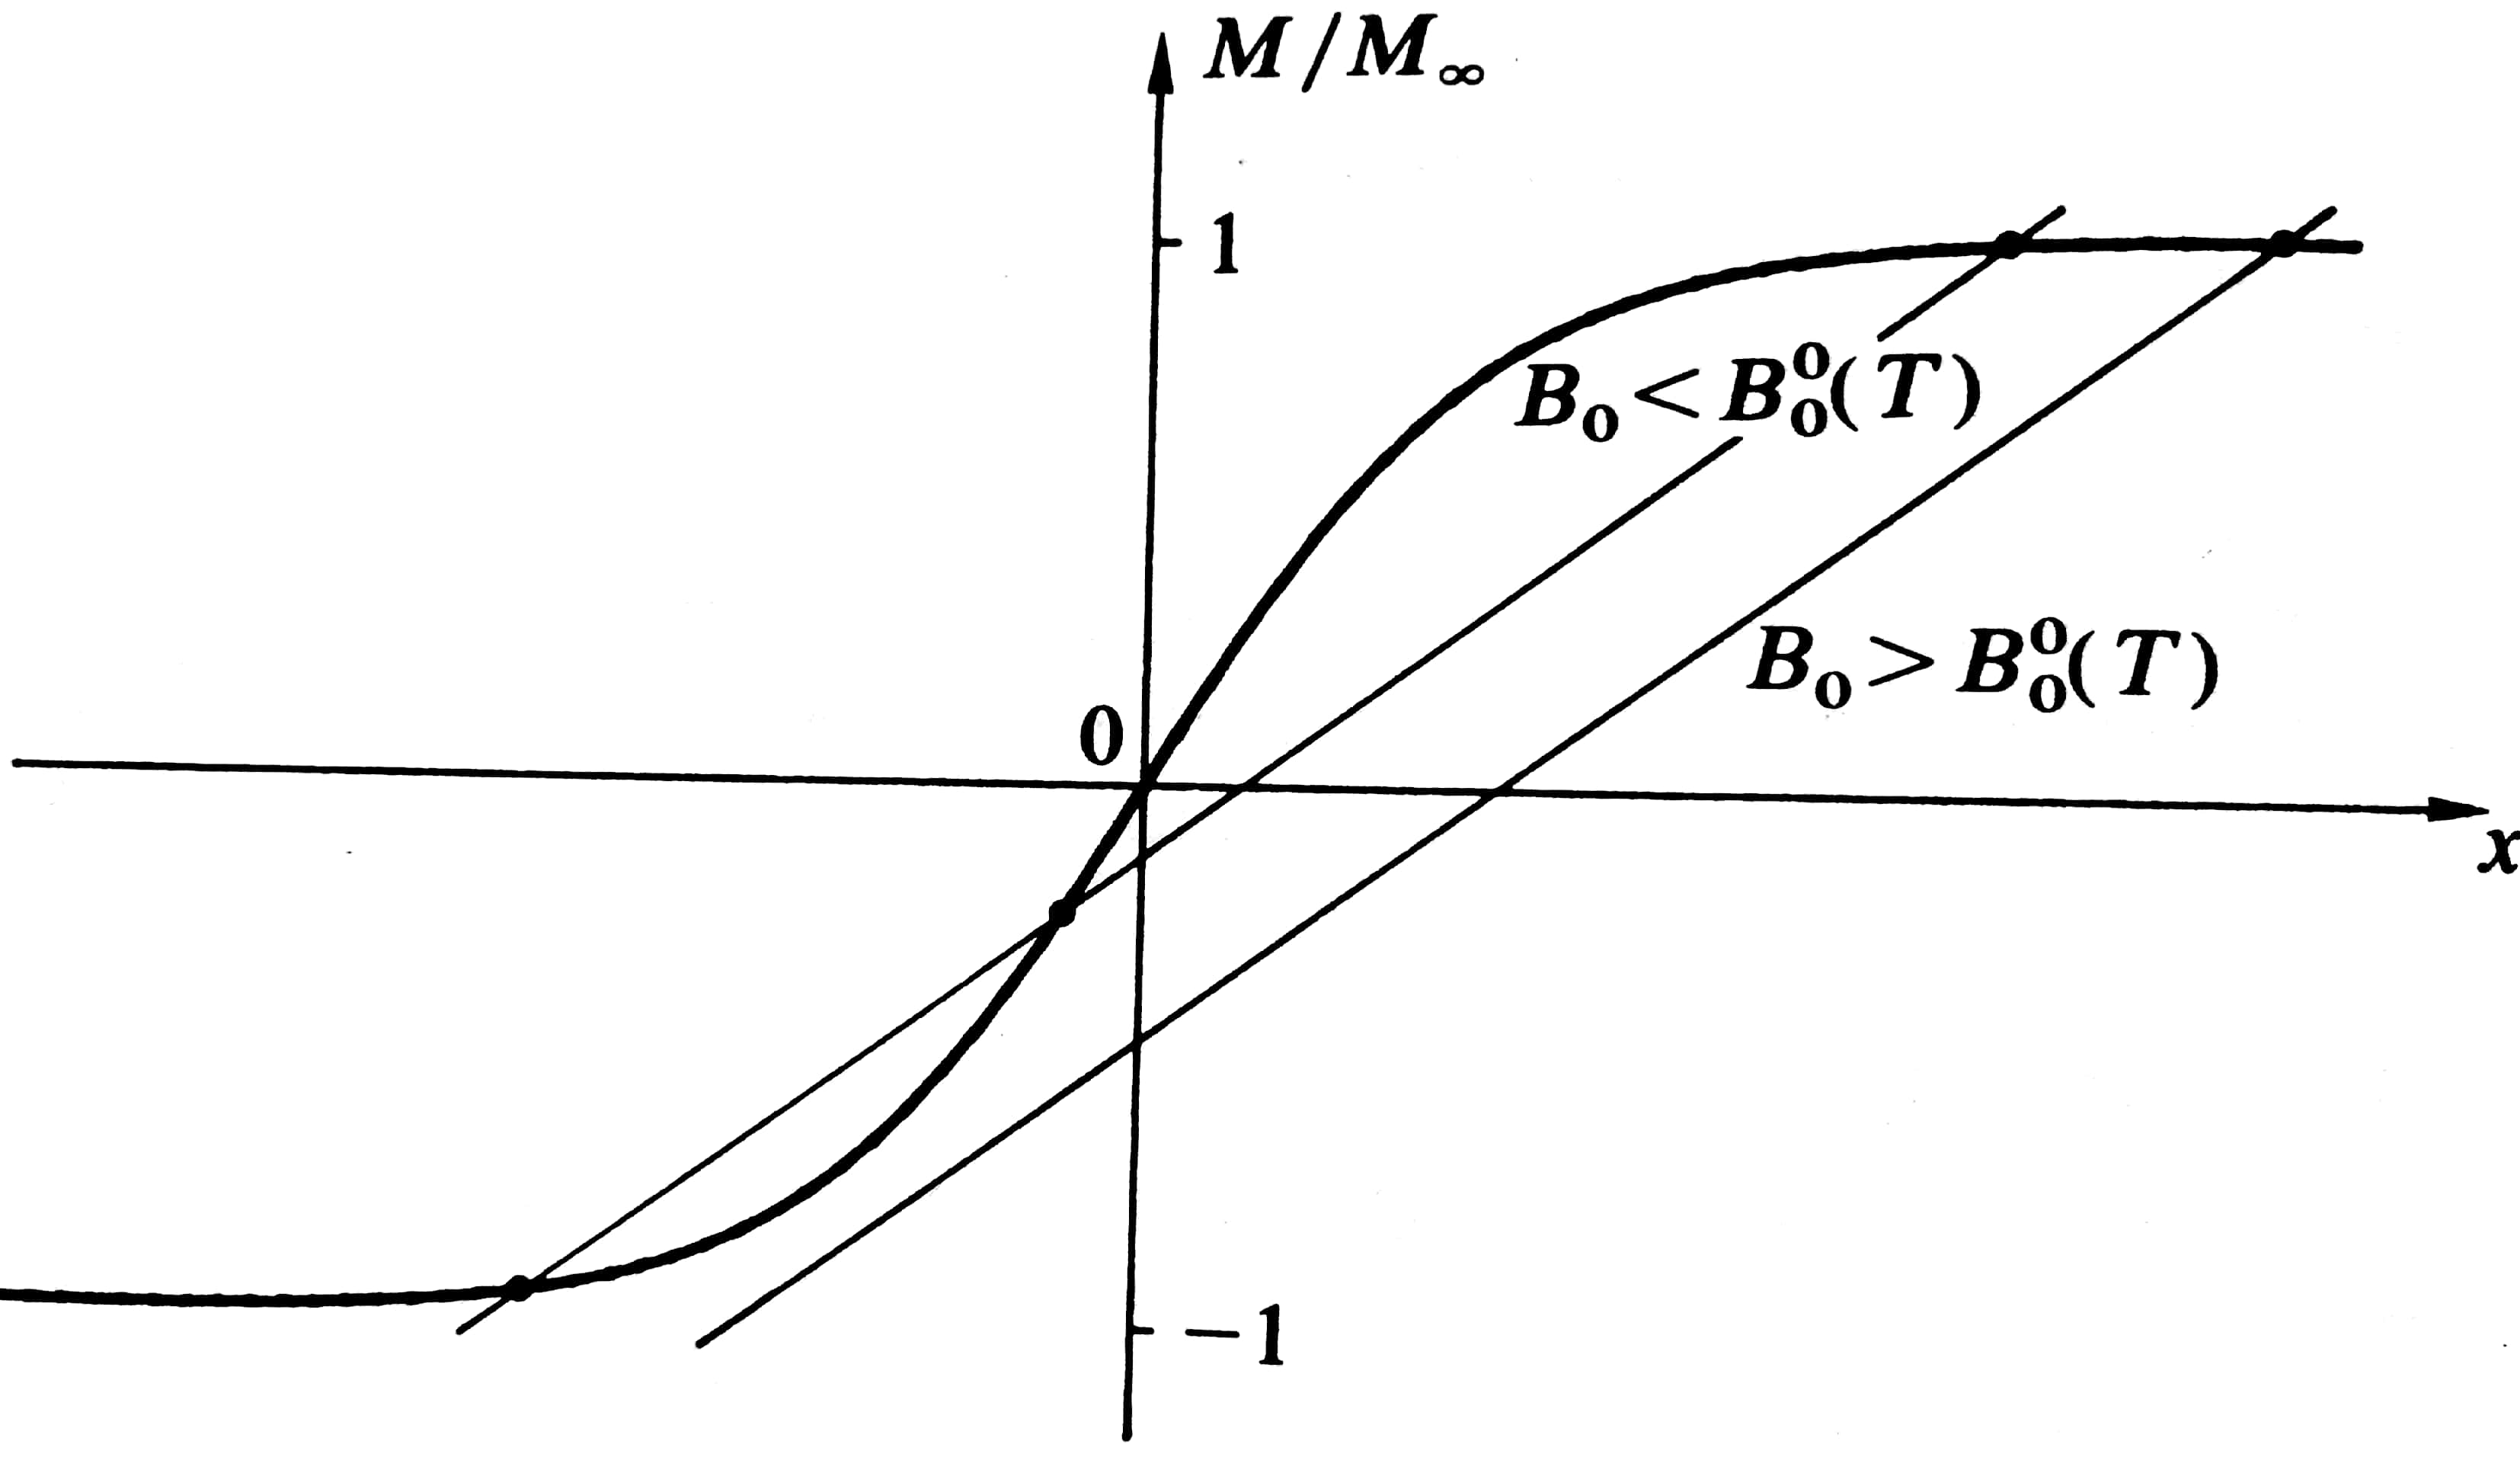
\includegraphics[width=6cm]{def_B0}
		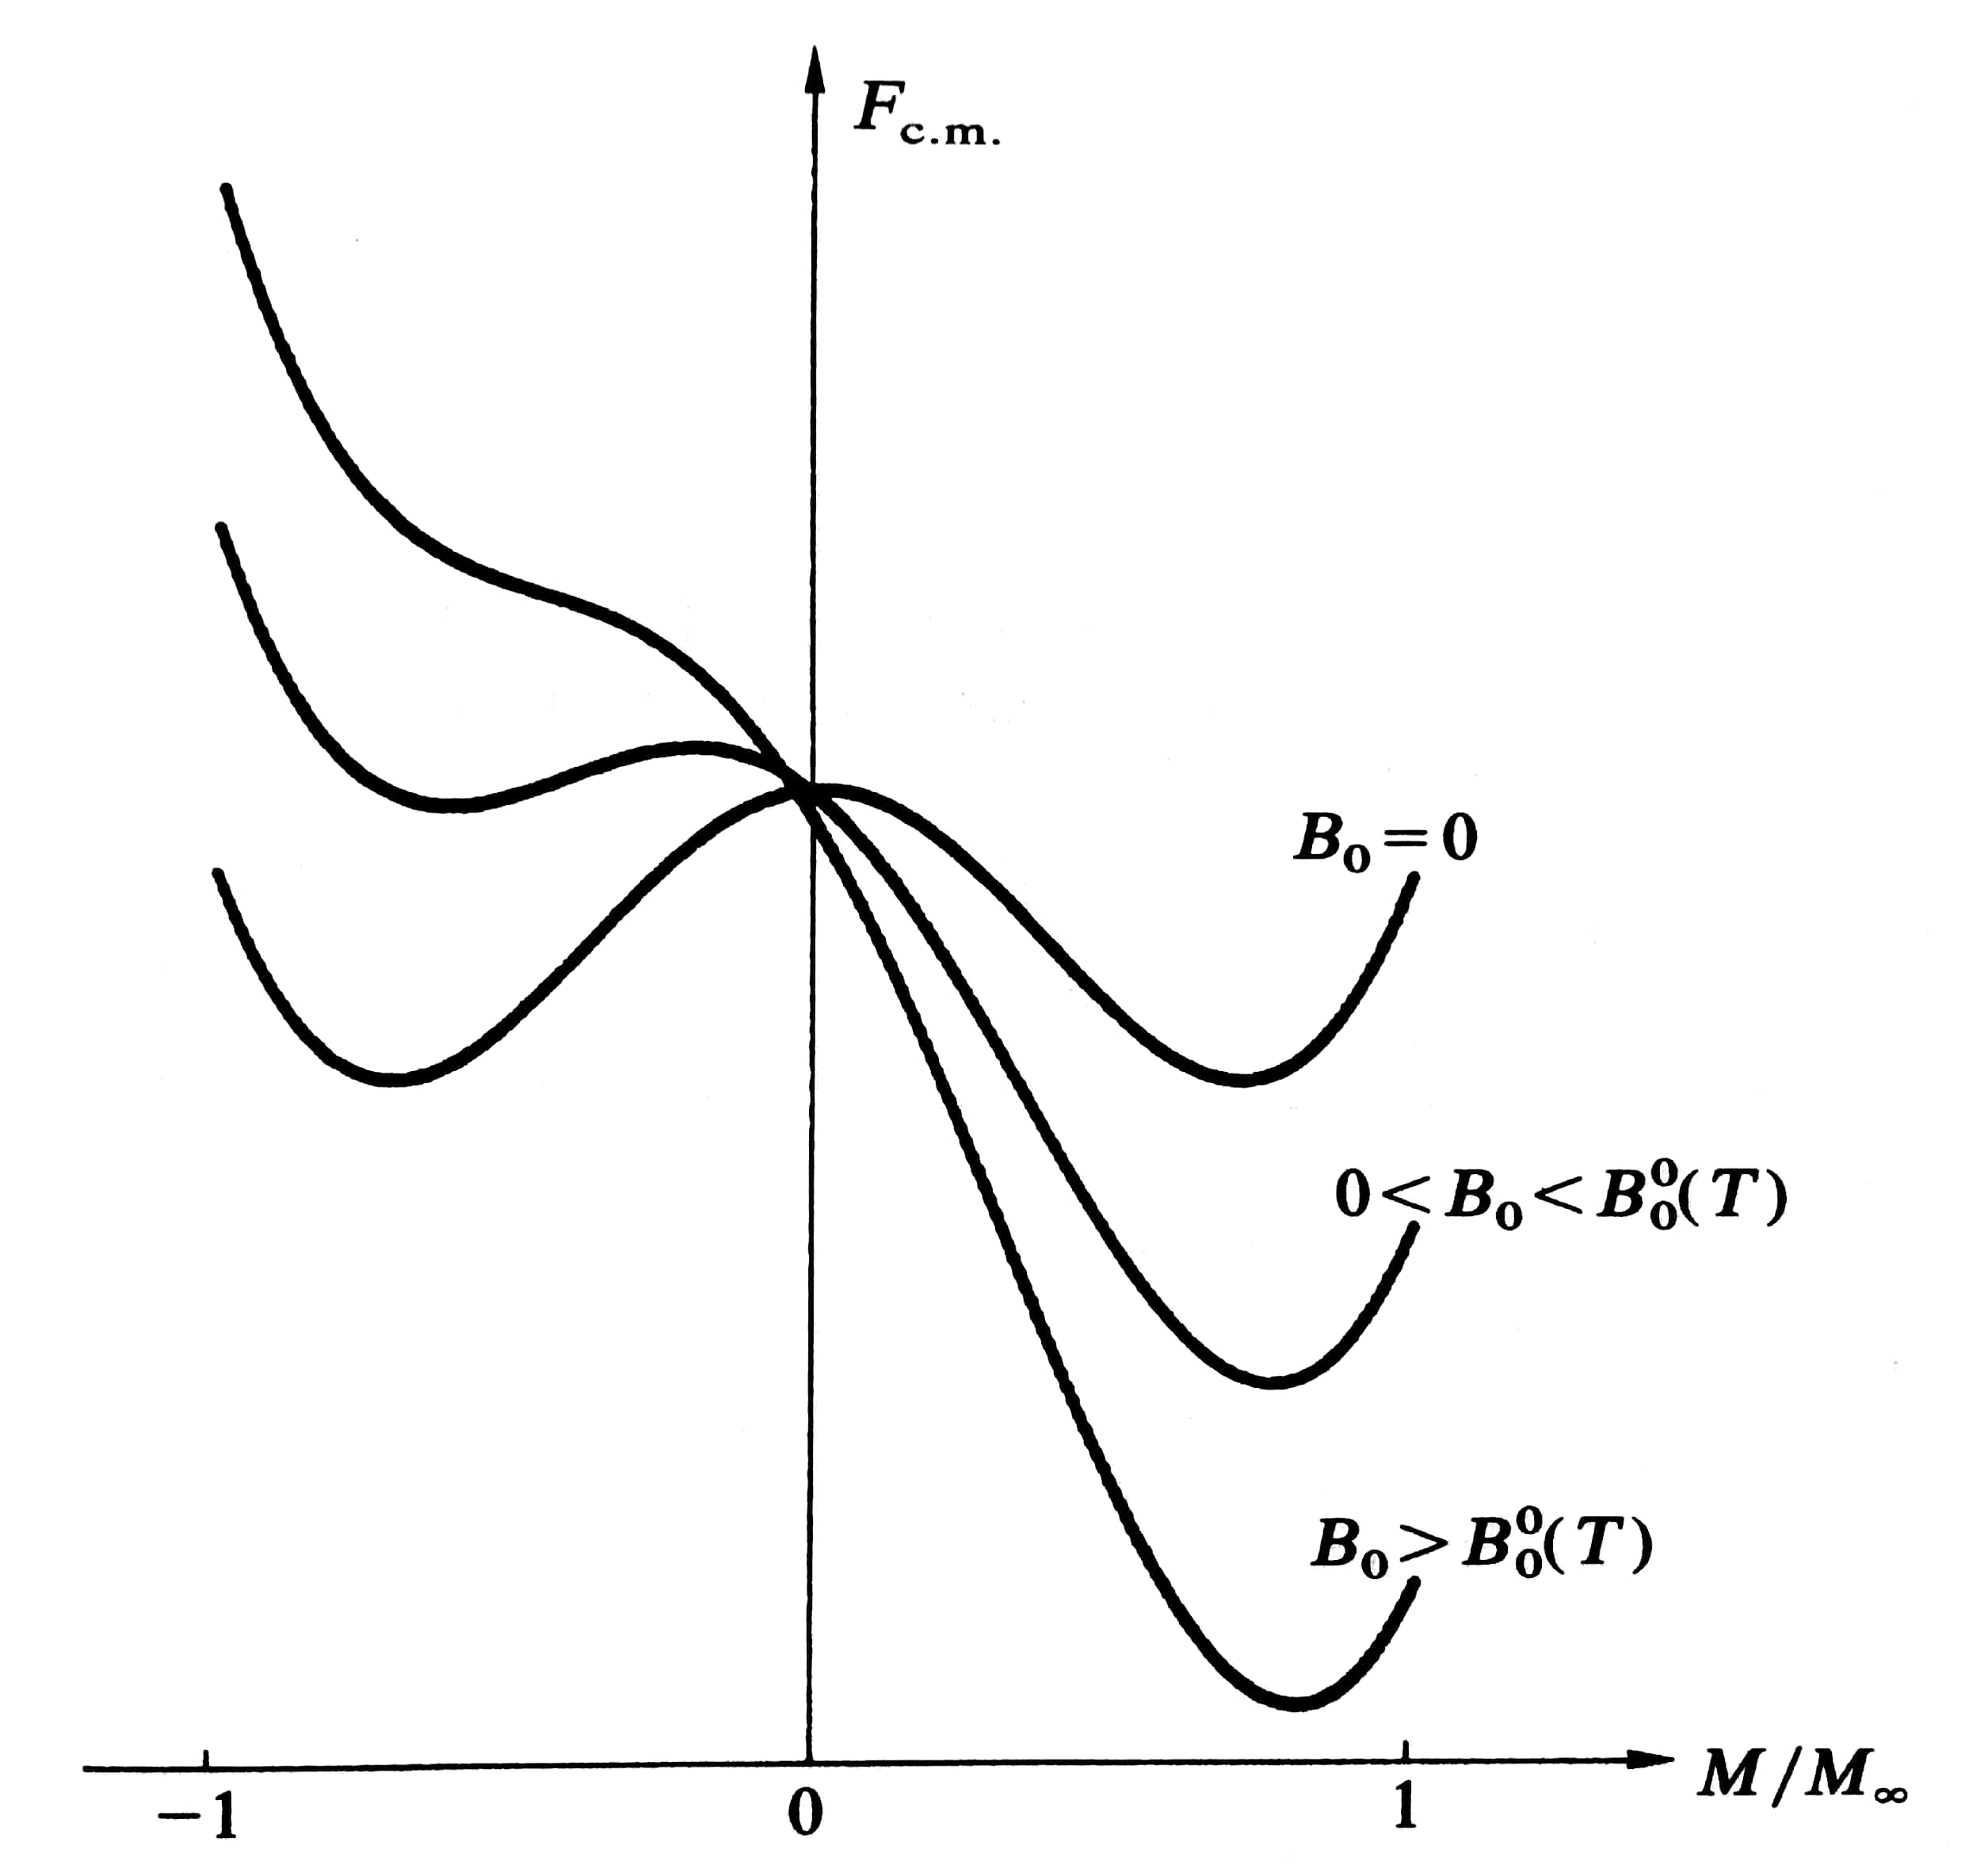
\includegraphics[width=5.5cm]{F_cas_general}}
\end{figure}
On voit que cela correspond bien au cycle d'hystérésis présenté au début de cette partie, notre modèle semble donc rendre compte du comportement observé. \\

On peut aussi comparer notre courbe de l'aimantation en fonction de la température avec des résultats expérimentaux :

\begin{figure}[h]
	\centerline{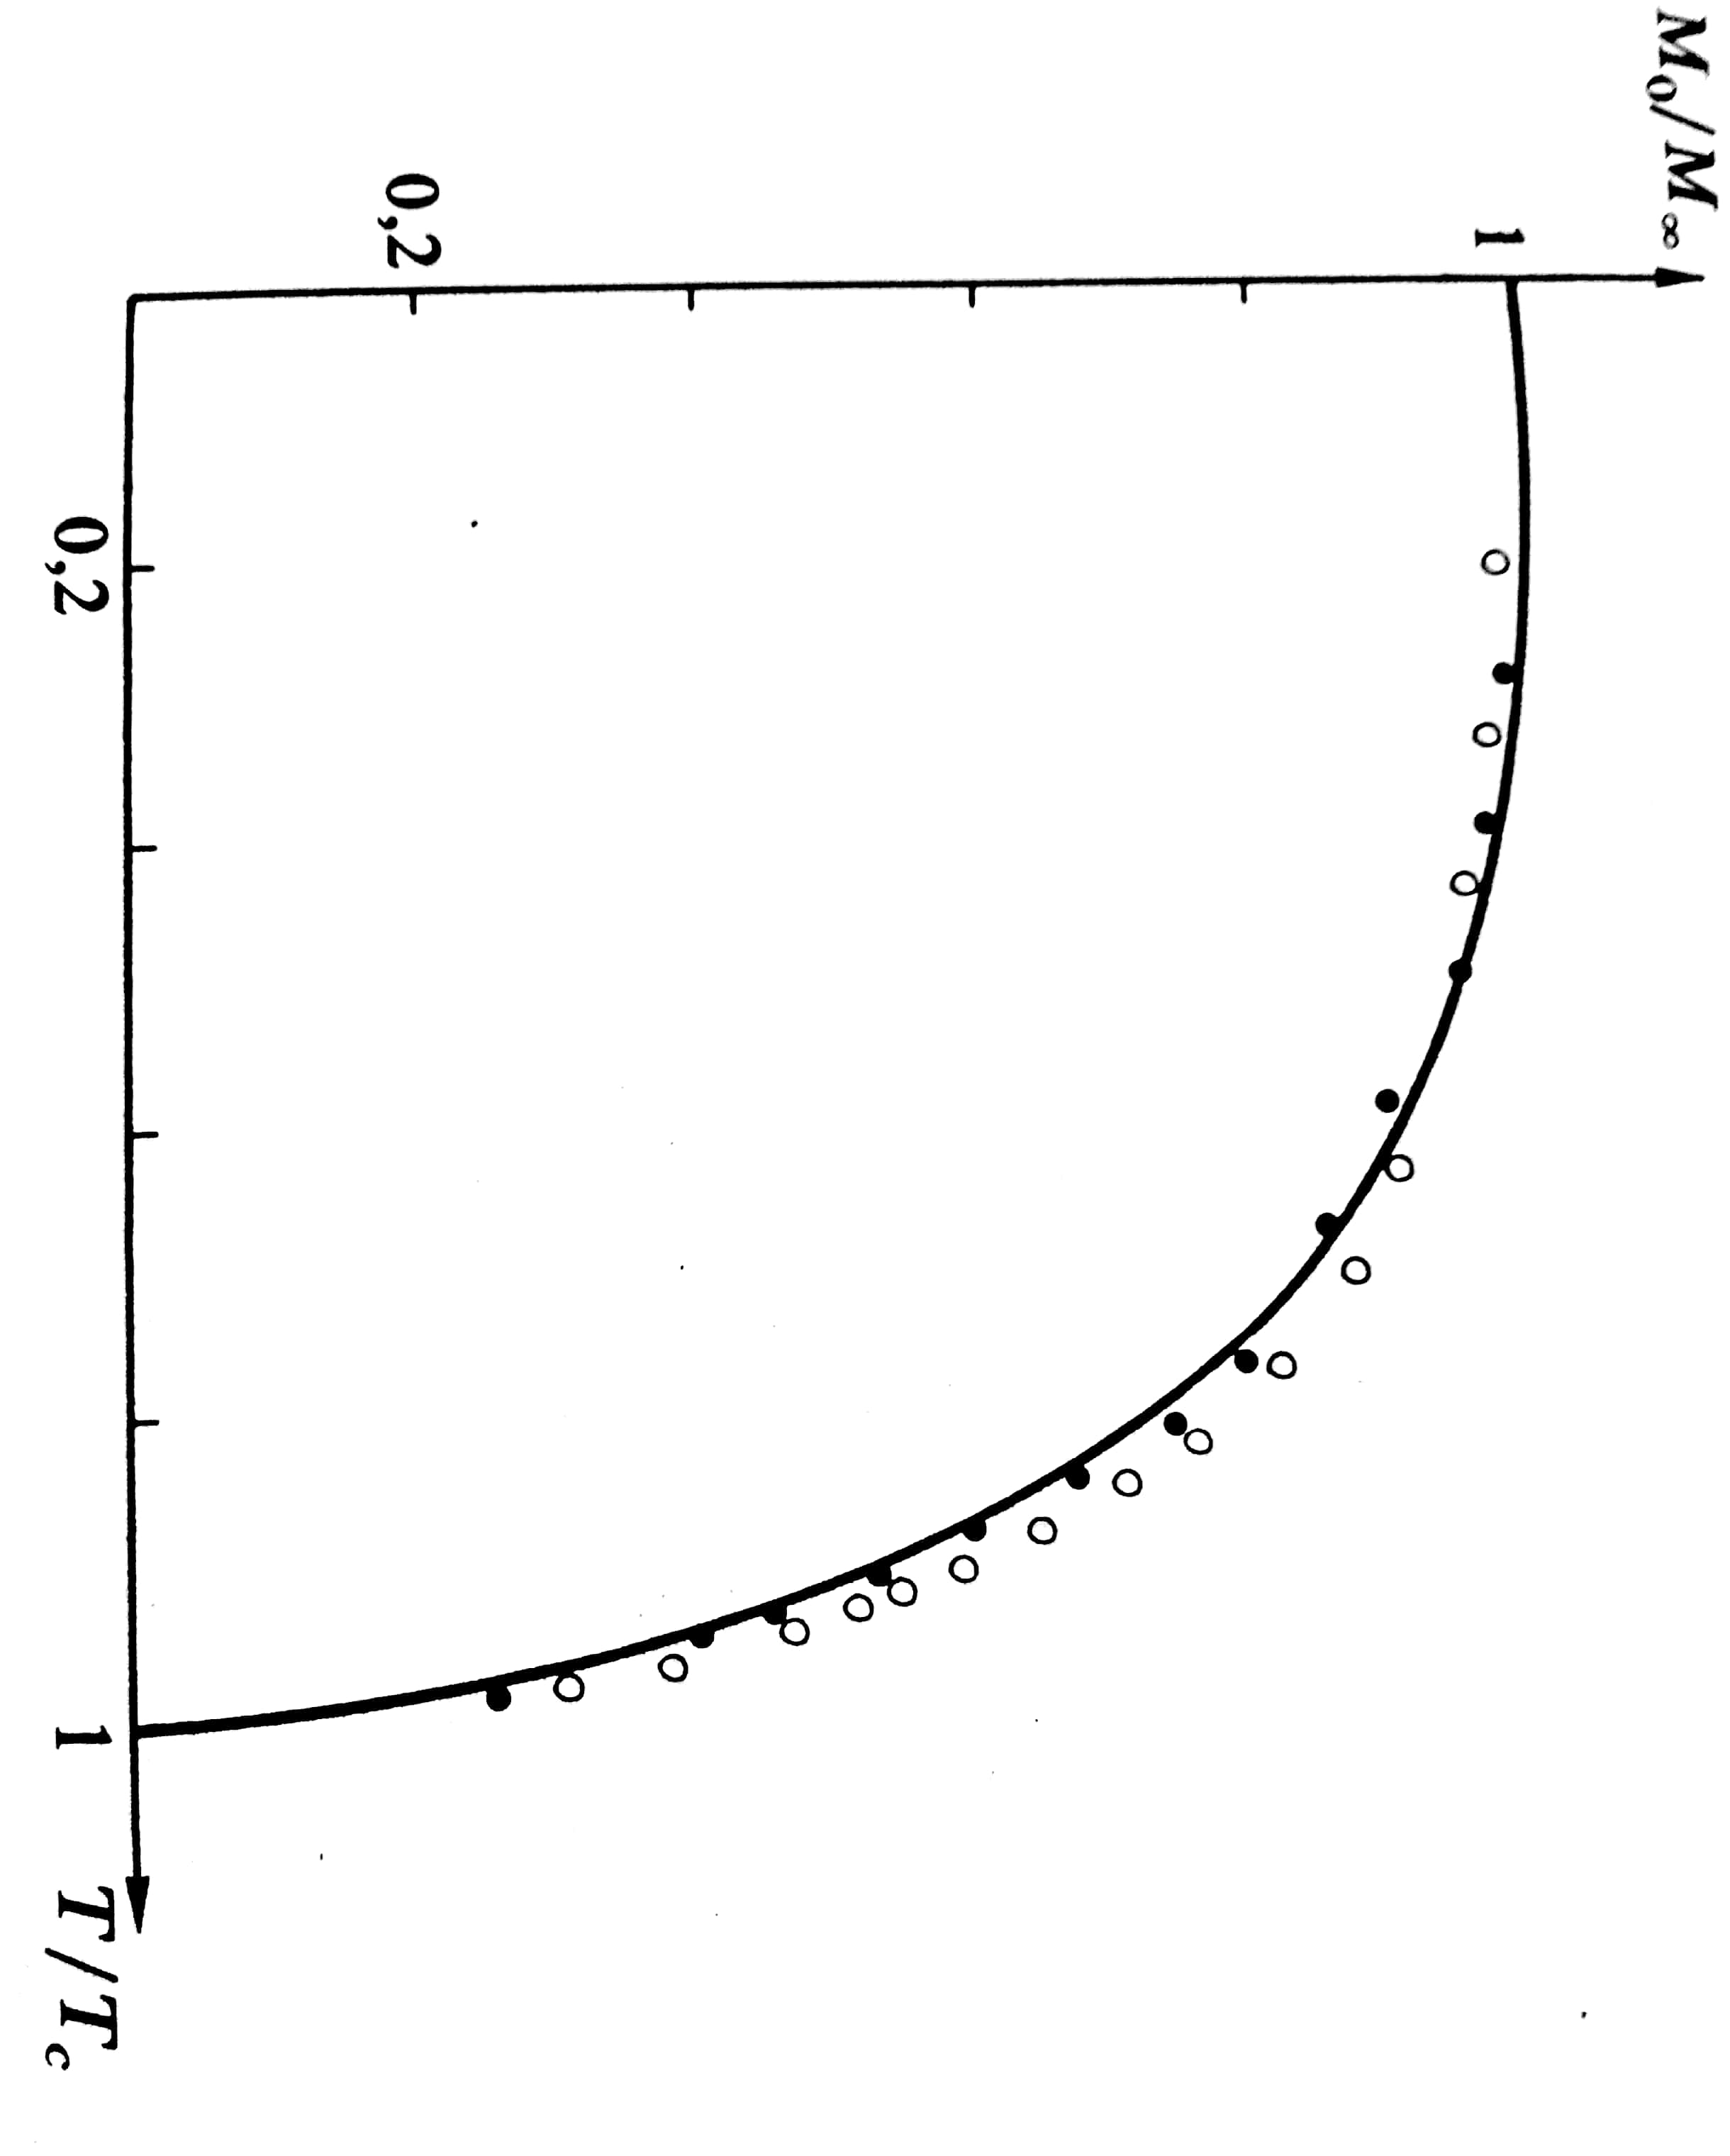
\includegraphics[width=8cm,angle=90]{comparaison}}

\end{figure}

avec les points noir pour le cobalt et nickel, et les blancs pour le fer. On constate alors que l'accord est excellent, si ce n'est pour $T\simeq T_c$ mais cela n'a rien de surprenant : c'est la zone où les fluctuations sont déterminantes, fluctuations que nous avons négligé en faisant l'approximation de champ moyen.
	
\section{Conclusion}
On a pu voir au cours de cette leçon comment on pouvait mêler thermodynamique, physique statistique, mécanique quantique et électromagnétisme pour expliquer, finalement assez simplement les deux comportements magnétiques que sont le paramagnétisme et le ferromagnétisme. L'approximation de champ moyen effectuée ne permet pas de rendre compte de toutes les subtilités du ferromagnétisme, mais une étude numérique du hamiltonien de Heisenberg peut permettre d'aller plus loin.

\section*{Questions}

\begin{itemize}
	
	\item Tu veux dire quoi par modèle Coulombien ? C'est quoi dipôle électrostatique ?
	\item unités de M et de m ? 
	\item Le moment cinétique L est lié à quoi ? 
	\item grandeur qui caractérise le dia et para et ferro ? susceptibilité. Ordre de grandeur ?
	\item relation entre J, S et L ?
	\item énergie spin, laquelle est l'énergie la plus basse ?
	\item pourquoi tu as montré le cycle d'hystérésis ? 
	\item hamiltonien, pourquoi j est positif ?
	\item graphe champ nul. Est-ce qu'avec ce graphe tu peut tracer l'aimantation en fonction de la température ? Tracer-le. Comment s'appelle le point qui coupe les ordonnées ? (Minf)
	\item pourquoi on ne parle pas du moment magnétique nucléaire ? Car le noyau est beaucoup plus lourd et alors le moment magnétique est beaucoup plus petit.
	\item différence entre para et ferro au niveau microscopique ? 
\end{itemize}

\section*{Remarques}
	préparer des questions sur les exposants critiques.\\
	Enlever la partie I.1, et définir M comme une densité de moment magnétique à la fin du I.2, ajouter une manip mettant en évidence transition ferro para en introduction pour motiver la leçon. Enlever l'introduction historique : la remplacer par manip + I.2\\
	Possibilité d'établir qualitativement la courbe $M(T)$ mettant en valeur la transition à partir de la courbe $\frac{M}{M_{\infty}}(x)$ en champ nul.
\end{document}